\pdfoutput=1
% Uncomment line above if submitting to arXiv and using pdflatex

% $Id: main.tex 124030 2018-10-12 09:08:33Z pkoppenb $
% ============================================================================
% Purpose: Template for LHCb documents
% Authors: Tomasz Skwarnicki, Roger Forty, Ulrik Egede
% Created on: 2010-09-24
% ============================================================================
\documentclass[12pt,a4paper]{article}
%%\documentclass[12pt,letter]{article}
% For two column text, add "twocolumn" as an option to the document
% class. Also uncomment the two "onecolumn" and "twocolumn" lines
% around the title page below.

% Variables that controls behaviour
\usepackage{ifthen} % for conditional statements
\newboolean{pdflatex}
\setboolean{pdflatex}{true} % False for eps figures 

\newboolean{articletitles}
\setboolean{articletitles}{true} % False removes titles in references

\newboolean{uprightparticles}
\setboolean{uprightparticles}{false} %True for upright particle symbols

%\newboolean{inbibliography}
%\setboolean{inbibliography}{false} %True once you enter the bibliography

% Define titles and authors here. It will then be used both in metadata and in
% what is printed on the front page.
\def\paperauthors{Wojciech Krupa$^1$} % Leave as is for PAPER and CONF
\def\paperasciititle{First observation of Bs -> Ds* K_s^0pi decay and  Bs -> Ds* K* decays} % Set ASCII title 
\def\papertitle{First observation of $\Bs\to\Dss\KS\pim$ and  $\Bs\to\Dss\Kstarm$ decays} % Latex formatted title
\def\paperkeywords{{High Energy Physics}, {LHCb}} % Comma separated list
%\def\papercopyright{CERN on behalf of the LHCb collaboration}
\def\papercopyright{\the\year\ CERN for the benefit of the LHCb collaboration} % new since 9/Apr/2018
\def\paperlicence{CC-BY-4.0 licence}
\def\paperlicenceurl{https://creativecommons.org/licenses/by/4.0/}


% THis file contains all the default packages and modifications for
% LHCb formatting

%% %%%%%%%%%%%%%%%%%%
%%  Page formatting
%% %%%%%%%%%%%%%%%%%%
%%\usepackage[margin=1in]{geometry}
\usepackage[top=1in, bottom=1.25in, left=1in, right=1in]{geometry}

% fallback for manual settings... uncomment if the geometry package is not available
%
%\voffset=-11mm
%\textheight=220mm
%\textwidth=160mm
%\oddsidemargin=0mm
%\evensidemargin=0mm

\columnsep=5mm
\addtolength{\belowcaptionskip}{0.5em}

\renewcommand{\textfraction}{0.01}
\renewcommand{\floatpagefraction}{0.8} % changed from 0.99
\renewcommand{\topfraction}{0.9}
\renewcommand{\bottomfraction}{0.9}

% Allow the page size to vary a bit ...
\raggedbottom
% To avoid Latex to be too fussy with line breaking ...
\sloppy

%% %%%%%%%%%%%%%%%%%%%%%%%
%% Packages to be used
%% %%%%%%%%%%%%%%%%%%%%%%% 
\usepackage{microtype}
\usepackage{lineno}  % for line numbering during review
\usepackage{xspace} % To avoid problems with missing or double spaces after
                    % predefined symbold
\usepackage{caption} %these three command get the figure and table captions automatically small
\renewcommand{\captionfont}{\small}
\renewcommand{\captionlabelfont}{\small}

%% Graphics
\usepackage{graphicx}  % to include figures (can also use other packages)
\usepackage{color}
\usepackage{colortbl}
\graphicspath{{./figs/}} % Make Latex search fig subdir for figures
\DeclareGraphicsExtensions{.pdf,.PDF,png,.PNG}

%% Math
\usepackage{amsmath} % Adds a large collection of math symbols
\usepackage{amssymb}
\usepackage{amsfonts}
\usepackage{upgreek} % Adds in support for greek letters in roman typeset

%% fix to allow peaceful coexistence of line numbering and
%% mathematical objects
%% http://www.latex-community.org/forum/viewtopic.php?f=5&t=163
%%
\newcommand*\patchAmsMathEnvironmentForLineno[1]{%
\expandafter\let\csname old#1\expandafter\endcsname\csname #1\endcsname
\expandafter\let\csname oldend#1\expandafter\endcsname\csname
end#1\endcsname
 \renewenvironment{#1}%
   {\linenomath\csname old#1\endcsname}%
   {\csname oldend#1\endcsname\endlinenomath}%
}
\newcommand*\patchBothAmsMathEnvironmentsForLineno[1]{%
  \patchAmsMathEnvironmentForLineno{#1}%
  \patchAmsMathEnvironmentForLineno{#1*}%
}
\AtBeginDocument{%
\patchBothAmsMathEnvironmentsForLineno{equation}%
\patchBothAmsMathEnvironmentsForLineno{align}%
\patchBothAmsMathEnvironmentsForLineno{flalign}%
\patchBothAmsMathEnvironmentsForLineno{alignat}%
\patchBothAmsMathEnvironmentsForLineno{gather}%
\patchBothAmsMathEnvironmentsForLineno{multline}%
\patchBothAmsMathEnvironmentsForLineno{eqnarray}%
}

% Get hyperlinks to captions and in references.
% These do not work with revtex. Use "hypertext" as class option instead.

\usepackage{hyperxmp}

\usepackage[pdftex,
            pdfauthor={\paperauthors},
            pdftitle={\paperasciititle},
            pdfkeywords={\paperkeywords},
            pdfcopyright={Copyright (C) \papercopyright},
            pdflicenseurl={\paperlicenceurl}]{hyperref}

% overleaf comments
\usepackage[colorinlistoftodos,textsize=scriptsize]{todonotes}

\usepackage[all]{hypcap} % Internal hyperlinks to floats.
%%% $Id: lhcb-symbols-def.tex 125058 2018-12-06 11:25:21Z pkoppenb $
%%% ======================================================================
%%% Purpose: Standard LHCb aliases
%%% Author: Originally Ulrik Egede, adapted by Tomasz Skwarnicki for templates,
%%% rewritten by Chris Parkes
%%% Maintainer : Ulrik Egede (2010 - 2012)
%%% Maintainer : Rolf Oldeman (2012 - 2014)
%%% Maintainer : Patrick Koppenburg (2018--2020)
%%% =======================================================================

%%% To use this file outside the normal LHCb document environment, the
%%% following should be added in a preamble (before \begin{document}
%%%
%%%\usepackage{ifthen} 
%%%\newboolean{uprightparticles}
%%%\setboolean{uprightparticles}{false} %Set true for upright particle symbols
\usepackage{xspace} 
\usepackage{upgreek}


%%%%%%%%%%%%%%%%%%%%%%%%%%%%%%%%%%%%%%%%%%%%%%%%%%%%%%%%%%%%
%%%
%%% The following is to ensure that the template automatically can process
%%% this file.
%%%
%%% Add comments with at least three %%% preceding.
%%% Add new sections with one % preceding
%%% Add new subsections with two %% preceding
%%%
%%% For upper greek letters, Xires and Xiresbar will be the particles without the charge
%%% States with charge are called Xiz and Xim  
%%%
%%%%%%%%%%%%%%%%%%%%%%%%%%%%%%%%%%%%%%%%%%%%%%%%%%%%%%%%%%%%

%%%%%%%%%%%%%
% Experiments
%%%%%%%%%%%%%
\def\lhcb   {\mbox{LHCb}\xspace}
\def\atlas  {\mbox{ATLAS}\xspace}
\def\cms    {\mbox{CMS}\xspace}
\def\alice  {\mbox{ALICE}\xspace}
\def\babar  {\mbox{BaBar}\xspace}
\def\belle  {\mbox{Belle}\xspace}
\def\belletwo {\mbox{Belle~II}\xspace}
\def\besiii {\mbox{BESIII}\xspace}
\def\cleo   {\mbox{CLEO}\xspace}
\def\cdf    {\mbox{CDF}\xspace}
\def\dzero  {\mbox{D0}\xspace}
\def\aleph  {\mbox{ALEPH}\xspace}
\def\delphi {\mbox{DELPHI}\xspace}
\def\opal   {\mbox{OPAL}\xspace}
\def\lthree {\mbox{L3}\xspace}
\def\sld    {\mbox{SLD}\xspace}
%%%\def\argus  {\mbox{ARGUS}\xspace}
%%%\def\uaone  {\mbox{UA1}\xspace}
%%%\def\uatwo  {\mbox{UA2}\xspace}
%%%\def\ux85 {\mbox{UX85}\xspace}
\def\cern {\mbox{CERN}\xspace}
\def\lhc    {\mbox{LHC}\xspace}
\def\lep    {\mbox{LEP}\xspace}
\def\tevatron {Tevatron\xspace}
\def\bfactories {\mbox{\B Factories}\xspace}
\def\bfactory   {\mbox{\B Factory}\xspace}
\def\upgradeone {\mbox{Upgrade~I}\xspace}
\def\upgradetwo {\mbox{Upgrade~II}\xspace}

%% LHCb sub-detectors and sub-systems

%%%\def\pu     {PU\xspace}
\def\velo   {VELO\xspace}
\def\rich   {RICH\xspace}
\def\richone {RICH1\xspace}
\def\richtwo {RICH2\xspace}
\def\ttracker {TT\xspace}
\def\intr   {IT\xspace}
\def\st     {ST\xspace}
\def\ot     {OT\xspace}
\def\herschel {\mbox{\textsc{HeRSCheL}}\xspace}
%%%\def\Tone   {T1\xspace}
%%%\def\Ttwo   {T2\xspace}
%%%\def\Tthree {T3\xspace}
%%%\def\Mone   {M1\xspace}
%%%\def\Mtwo   {M2\xspace}
%%%\def\Mthree {M3\xspace}
%%%\def\Mfour  {M4\xspace}
%%%\def\Mfive  {M5\xspace}
\def\spd    {SPD\xspace}
\def\presh  {PS\xspace}
\def\ecal   {ECAL\xspace}
\def\hcal   {HCAL\xspace}
%%%\def\bcm    {BCM\xspace}
\def\MagUp {\mbox{\em Mag\kern -0.05em Up}\xspace}
\def\MagDown {\mbox{\em MagDown}\xspace}

\def\ode    {ODE\xspace}
\def\daq    {DAQ\xspace}
\def\tfc    {TFC\xspace}
\def\ecs    {ECS\xspace}
\def\lone   {L0\xspace}
\def\hlt    {HLT\xspace}
\def\hltone {HLT1\xspace}
\def\hlttwo {HLT2\xspace}

%%% Upright (not slanted) Particles

\ifthenelse{\boolean{uprightparticles}}%
{\def\Palpha      {\ensuremath{\upalpha}\xspace}
 \def\Pbeta       {\ensuremath{\upbeta}\xspace}
 \def\Pgamma      {\ensuremath{\upgamma}\xspace}                 
 \def\Pdelta      {\ensuremath{\updelta}\xspace}                 
 \def\Pepsilon    {\ensuremath{\upepsilon}\xspace}                 
 \def\Pvarepsilon {\ensuremath{\upvarepsilon}\xspace}                 
 \def\Pzeta       {\ensuremath{\upzeta}\xspace}                 
 \def\Peta        {\ensuremath{\upeta}\xspace}
 \def\Ptheta      {\ensuremath{\uptheta}\xspace}                 
 \def\Pvartheta   {\ensuremath{\upvartheta}\xspace}                 
 \def\Piota       {\ensuremath{\upiota}\xspace}                 
 \def\Pkappa      {\ensuremath{\upkappa}\xspace}                 
 \def\Plambda     {\ensuremath{\uplambda}\xspace}                 
 \def\Pmu         {\ensuremath{\upmu}\xspace}                 
 \def\Pnu         {\ensuremath{\upnu}\xspace}                 
 \def\Pxi         {\ensuremath{\upxi}\xspace}                 
 \def\Ppi         {\ensuremath{\uppi}\xspace}                 
 \def\Pvarpi      {\ensuremath{\upvarpi}\xspace}                 
 \def\Prho        {\ensuremath{\uprho}\xspace}                 
 \def\Pvarrho     {\ensuremath{\upvarrho}\xspace}                 
 \def\Ptau        {\ensuremath{\uptau}\xspace}                 
 \def\Pupsilon    {\ensuremath{\upupsilon}\xspace}                 
 \def\Pphi        {\ensuremath{\upphi}\xspace}                 
 \def\Pvarphi     {\ensuremath{\upvarphi}\xspace}                 
 \def\Pchi        {\ensuremath{\upchi}\xspace}                 
 \def\Ppsi        {\ensuremath{\uppsi}\xspace}                 
 \def\Pomega      {\ensuremath{\upomega}\xspace}                 

 \def\PDelta      {\ensuremath{\Delta}\xspace}                 
 \def\PXi         {\ensuremath{\Xi}\xspace}                 
 \def\PLambda     {\ensuremath{\Lambda}\xspace}                 
 \def\PSigma      {\ensuremath{\Sigma}\xspace}                 
 \def\POmega      {\ensuremath{\Omega}\xspace}                 
 \def\PUpsilon    {\ensuremath{\Upsilon}\xspace}                 

 \def\PA      {\ensuremath{\mathrm{A}}\xspace}                 
 \def\PB      {\ensuremath{\mathrm{B}}\xspace}                 
 \def\PC      {\ensuremath{\mathrm{C}}\xspace}                 
 \def\PD      {\ensuremath{\mathrm{D}}\xspace}                 
 \def\PE      {\ensuremath{\mathrm{E}}\xspace}                 
 \def\PF      {\ensuremath{\mathrm{F}}\xspace}                 
 \def\PG      {\ensuremath{\mathrm{G}}\xspace}                 
 \def\PH      {\ensuremath{\mathrm{H}}\xspace}                 
 \def\PI      {\ensuremath{\mathrm{I}}\xspace}                 
 \def\PJ      {\ensuremath{\mathrm{J}}\xspace}                 
 \def\PK      {\ensuremath{\mathrm{K}}\xspace}                 
 \def\PL      {\ensuremath{\mathrm{L}}\xspace}                 
 \def\PM      {\ensuremath{\mathrm{M}}\xspace}                 
 \def\PN      {\ensuremath{\mathrm{N}}\xspace}                 
 \def\PO      {\ensuremath{\mathrm{O}}\xspace}                 
 \def\PP      {\ensuremath{\mathrm{P}}\xspace}                 
 \def\PQ      {\ensuremath{\mathrm{Q}}\xspace}                 
 \def\PR      {\ensuremath{\mathrm{R}}\xspace}                 
 \def\PS      {\ensuremath{\mathrm{S}}\xspace}                 
 \def\PT      {\ensuremath{\mathrm{T}}\xspace}                 
 \def\PU      {\ensuremath{\mathrm{U}}\xspace}                 
 \def\PV      {\ensuremath{\mathrm{V}}\xspace}                 
 \def\PW      {\ensuremath{\mathrm{W}}\xspace}                 
 \def\PX      {\ensuremath{\mathrm{X}}\xspace}                 
 \def\PY      {\ensuremath{\mathrm{Y}}\xspace}                 
 \def\PZ      {\ensuremath{\mathrm{Z}}\xspace}                 
 \def\Pa      {\ensuremath{\mathrm{a}}\xspace}                 
 \def\Pb      {\ensuremath{\mathrm{b}}\xspace}                 
 \def\Pc      {\ensuremath{\mathrm{c}}\xspace}                 
 \def\Pd      {\ensuremath{\mathrm{d}}\xspace}                 
 \def\Pe      {\ensuremath{\mathrm{e}}\xspace}                 
 \def\Pf      {\ensuremath{\mathrm{f}}\xspace}                 
 \def\Pg      {\ensuremath{\mathrm{g}}\xspace}                 
 \def\Ph      {\ensuremath{\mathrm{h}}\xspace}                 
 \def\Pi      {\ensuremath{\mathrm{i}}\xspace}                 
 \def\Pj      {\ensuremath{\mathrm{j}}\xspace}                 
 \def\Pk      {\ensuremath{\mathrm{k}}\xspace}                 
 \def\Pl      {\ensuremath{\mathrm{l}}\xspace}                 
 \def\Pm      {\ensuremath{\mathrm{m}}\xspace}                 
 \def\Pn      {\ensuremath{\mathrm{n}}\xspace}                 
 \def\Po      {\ensuremath{\mathrm{o}}\xspace}                 
 \def\Pp      {\ensuremath{\mathrm{p}}\xspace}                 
 \def\Pq      {\ensuremath{\mathrm{q}}\xspace}                 
 \def\Pr      {\ensuremath{\mathrm{r}}\xspace}                 
 \def\Ps      {\ensuremath{\mathrm{s}}\xspace}                 
 \def\Pt      {\ensuremath{\mathrm{t}}\xspace}                 
 \def\Pu      {\ensuremath{\mathrm{u}}\xspace}                 
 \def\Pv      {\ensuremath{\mathrm{v}}\xspace}                 
 \def\Pw      {\ensuremath{\mathrm{w}}\xspace}                 
 \def\Px      {\ensuremath{\mathrm{x}}\xspace}                 
 \def\Py      {\ensuremath{\mathrm{y}}\xspace}                 
 \def\Pz      {\ensuremath{\mathrm{z}}\xspace}                 
 \def\thebaroffset{0.0em}
}
{\def\Palpha      {\ensuremath{\alpha}\xspace}
 \def\Pbeta       {\ensuremath{\beta}\xspace}
 \def\Pgamma      {\ensuremath{\gamma}\xspace}                 
 \def\Pdelta      {\ensuremath{\delta}\xspace}                 
 \def\Pepsilon    {\ensuremath{\epsilon}\xspace}                 
 \def\Pvarepsilon {\ensuremath{\varepsilon}\xspace}                 
 \def\Pzeta       {\ensuremath{\zeta}\xspace}                 
 \def\Peta        {\ensuremath{\eta}\xspace}                 
 \def\Ptheta      {\ensuremath{\theta}\xspace}                 
 \def\Pvartheta   {\ensuremath{\vartheta}\xspace}                 
 \def\Piota       {\ensuremath{\iota}\xspace}                 
 \def\Pkappa      {\ensuremath{\kappa}\xspace}                 
 \def\Plambda     {\ensuremath{\lambda}\xspace}                 
 \def\Pmu         {\ensuremath{\mu}\xspace}                 
 \def\Pnu         {\ensuremath{\nu}\xspace}                 
 \def\Pxi         {\ensuremath{\xi}\xspace}                 
 \def\Ppi         {\ensuremath{\pi}\xspace}                 
 \def\Pvarpi      {\ensuremath{\varpi}\xspace}                 
 \def\Prho        {\ensuremath{\rho}\xspace}                 
 \def\Pvarrho     {\ensuremath{\varrho}\xspace}                 
 \def\Ptau        {\ensuremath{\tau}\xspace}                 
 \def\Pupsilon    {\ensuremath{\upsilon}\xspace}                 
 \def\Pphi        {\ensuremath{\phi}\xspace}                 
 \def\Pvarphi     {\ensuremath{\varphi}\xspace}                 
 \def\Pchi        {\ensuremath{\chi}\xspace}                 
 \def\Ppsi        {\ensuremath{\psi}\xspace}                 
 \def\Pomega      {\ensuremath{\omega}\xspace}                 
 \mathchardef\PDelta="7101
 \mathchardef\PXi="7104
 \mathchardef\PLambda="7103
 \mathchardef\PSigma="7106
 \mathchardef\POmega="710A
 \mathchardef\PUpsilon="7107
 \def\PA      {\ensuremath{A}\xspace}                 
 \def\PB      {\ensuremath{B}\xspace}                 
 \def\PC      {\ensuremath{C}\xspace}                 
 \def\PD      {\ensuremath{D}\xspace}                 
 \def\PE      {\ensuremath{E}\xspace}                 
 \def\PF      {\ensuremath{F}\xspace}                 
 \def\PG      {\ensuremath{G}\xspace}                 
 \def\PH      {\ensuremath{H}\xspace}                 
 \def\PI      {\ensuremath{I}\xspace}                 
 \def\PJ      {\ensuremath{J}\xspace}                 
 \def\PK      {\ensuremath{K}\xspace}                 
 \def\PL      {\ensuremath{L}\xspace}                 
 \def\PM      {\ensuremath{M}\xspace}                 
 \def\PN      {\ensuremath{N}\xspace}                 
 \def\PO      {\ensuremath{O}\xspace}                 
 \def\PP      {\ensuremath{P}\xspace}                 
 \def\PQ      {\ensuremath{Q}\xspace}                 
 \def\PR      {\ensuremath{R}\xspace}                 
 \def\PS      {\ensuremath{S}\xspace}                 
 \def\PT      {\ensuremath{T}\xspace}                 
 \def\PU      {\ensuremath{U}\xspace}                 
 \def\PV      {\ensuremath{V}\xspace}                 
 \def\PW      {\ensuremath{W}\xspace}                 
 \def\PX      {\ensuremath{X}\xspace}                 
 \def\PY      {\ensuremath{Y}\xspace}                 
 \def\PZ      {\ensuremath{Z}\xspace}                 
 \def\Pa      {\ensuremath{a}\xspace}                 
 \def\Pb      {\ensuremath{b}\xspace}                 
 \def\Pc      {\ensuremath{c}\xspace}                 
 \def\Pd      {\ensuremath{d}\xspace}                 
 \def\Pe      {\ensuremath{e}\xspace}                 
 \def\Pf      {\ensuremath{f}\xspace}                 
 \def\Pg      {\ensuremath{g}\xspace}                 
 \def\Ph      {\ensuremath{h}\xspace}                 
 \def\Pi      {\ensuremath{i}\xspace}                 
 \def\Pj      {\ensuremath{j}\xspace}                 
 \def\Pk      {\ensuremath{k}\xspace}                 
 \def\Pl      {\ensuremath{l}\xspace}                 
 \def\Pm      {\ensuremath{m}\xspace}                 
 \def\Pn      {\ensuremath{n}\xspace}                 
 \def\Po      {\ensuremath{o}\xspace}                 
 \def\Pp      {\ensuremath{p}\xspace}                 
 \def\Pq      {\ensuremath{q}\xspace}                 
 \def\Pr      {\ensuremath{r}\xspace}                 
 \def\Ps      {\ensuremath{s}\xspace}                 
 \def\Pt      {\ensuremath{t}\xspace}                 
 \def\Pu      {\ensuremath{u}\xspace}                 
 \def\Pv      {\ensuremath{v}\xspace}                 
 \def\Pw      {\ensuremath{w}\xspace}                 
 \def\Px      {\ensuremath{x}\xspace}                 
 \def\Py      {\ensuremath{y}\xspace}                 
 \def\Pz      {\ensuremath{z}\xspace}
 \def\thebaroffset{0.18em}
}
\newcommand{\offsetoverline}[2][\thebaroffset]{\kern #1\overline{\kern -#1 #2}}%

%%%%%%%%%%%%%%%%%%%%%%%%%%%%%%%%%%%%%%%%%%%%%%%
% Particles
\makeatletter
\ifcase \@ptsize \relax% 10pt
  \newcommand{\miniscule}{\@setfontsize\miniscule{4}{5}}% \tiny: 5/6
\or% 11pt
  \newcommand{\miniscule}{\@setfontsize\miniscule{5}{6}}% \tiny: 6/7
\or% 12pt
  \newcommand{\miniscule}{\@setfontsize\miniscule{5}{6}}% \tiny: 6/7
\fi
\makeatother


\DeclareRobustCommand{\optbar}[1]{\shortstack{{\miniscule (\rule[.5ex]{1.25em}{.18mm})}
  \\ [-.7ex] $#1$}}


%% Leptons

\let\emi\en
\def\electron   {{\ensuremath{\Pe}}\xspace}
\def\en         {{\ensuremath{\Pe^-}}\xspace}   % electron negative (\em is taken)
\def\ep         {{\ensuremath{\Pe^+}}\xspace}
\def\epm        {{\ensuremath{\Pe^\pm}}\xspace} 
\def\emp        {{\ensuremath{\Pe^\mp}}\xspace} 
\def\epem       {{\ensuremath{\Pe^+\Pe^-}}\xspace}
%%%\def\ee         {\ensuremath{\Pe^-\Pe^-}\xspace}

\def\muon       {{\ensuremath{\Pmu}}\xspace}
\def\mup        {{\ensuremath{\Pmu^+}}\xspace}
\def\mun        {{\ensuremath{\Pmu^-}}\xspace} % muon negative (\mum is taken)
\def\mupm       {{\ensuremath{\Pmu^\pm}}\xspace} 
\def\mump       {{\ensuremath{\Pmu^\mp}}\xspace} 
\def\mumu       {{\ensuremath{\Pmu^+\Pmu^-}}\xspace}

\def\tauon      {{\ensuremath{\Ptau}}\xspace}
\def\taup       {{\ensuremath{\Ptau^+}}\xspace}
\def\taum       {{\ensuremath{\Ptau^-}}\xspace}
\def\taupm      {{\ensuremath{\Ptau^\pm}}\xspace}
\def\taump      {{\ensuremath{\Ptau^\mp}}\xspace}
\def\tautau     {{\ensuremath{\Ptau^+\Ptau^-}}\xspace}

\def\lepton     {{\ensuremath{\ell}}\xspace}
\def\ellm       {{\ensuremath{\ell^-}}\xspace}
\def\ellp       {{\ensuremath{\ell^+}}\xspace}
\def\ellell     {\ensuremath{\ell^+ \ell^-}\xspace}

\def\neu        {{\ensuremath{\Pnu}}\xspace}
\def\neub       {{\ensuremath{\overline{\Pnu}}}\xspace}
%%%\def\nuenueb    {\ensuremath{\neu\neub}\xspace}
\def\neue       {{\ensuremath{\neu_e}}\xspace}
\def\neueb      {{\ensuremath{\neub_e}}\xspace}
%%%\def\neueneueb  {\ensuremath{\neue\neueb}\xspace}
\def\neum       {{\ensuremath{\neu_\mu}}\xspace}
\def\neumb      {{\ensuremath{\neub_\mu}}\xspace}
%%%\def\neumneumb  {\ensuremath{\neum\neumb}\xspace}
\def\neut       {{\ensuremath{\neu_\tau}}\xspace}
\def\neutb      {{\ensuremath{\neub_\tau}}\xspace}
%%%\def\neutneutb  {\ensuremath{\neut\neutb}\xspace}
\def\neul       {{\ensuremath{\neu_\ell}}\xspace}
\def\neulb      {{\ensuremath{\neub_\ell}}\xspace}
%%%\def\neulneulb  {\ensuremath{\neul\neulb}\xspace}

%% Gauge bosons and scalars

\def\g      {{\ensuremath{\Pgamma}}\xspace}
\def\H      {{\ensuremath{\PH^0}}\xspace}
\def\Hp     {{\ensuremath{\PH^+}}\xspace}
\def\Hm     {{\ensuremath{\PH^-}}\xspace}
\def\Hpm    {{\ensuremath{\PH^\pm}}\xspace}
\def\W      {{\ensuremath{\PW}}\xspace}
\def\Wp     {{\ensuremath{\PW^+}}\xspace}
\def\Wm     {{\ensuremath{\PW^-}}\xspace}
\def\Wpm    {{\ensuremath{\PW^\pm}}\xspace}
\def\Z      {{\ensuremath{\PZ}}\xspace}

%% Quarks

\def\quark     {{\ensuremath{\Pq}}\xspace}
\def\quarkbar  {{\ensuremath{\overline \quark}}\xspace}
\def\qqbar     {{\ensuremath{\quark\quarkbar}}\xspace}
\def\uquark    {{\ensuremath{\Pu}}\xspace}
\def\uquarkbar {{\ensuremath{\overline \uquark}}\xspace}
\def\uubar     {{\ensuremath{\uquark\uquarkbar}}\xspace}
\def\dquark    {{\ensuremath{\Pd}}\xspace}
\def\dquarkbar {{\ensuremath{\overline \dquark}}\xspace}
\def\ddbar     {{\ensuremath{\dquark\dquarkbar}}\xspace}
\def\squark    {{\ensuremath{\Ps}}\xspace}
\def\squarkbar {{\ensuremath{\overline \squark}}\xspace}
\def\ssbar     {{\ensuremath{\squark\squarkbar}}\xspace}
\def\cquark    {{\ensuremath{\Pc}}\xspace}
\def\cquarkbar {{\ensuremath{\overline \cquark}}\xspace}
\def\ccbar     {{\ensuremath{\cquark\cquarkbar}}\xspace}
\def\bquark    {{\ensuremath{\Pb}}\xspace}
\def\bquarkbar {{\ensuremath{\overline \bquark}}\xspace}
\def\bbbar     {{\ensuremath{\bquark\bquarkbar}}\xspace}
\def\tquark    {{\ensuremath{\Pt}}\xspace}
\def\tquarkbar {{\ensuremath{\overline \tquark}}\xspace}
\def\ttbar     {{\ensuremath{\tquark\tquarkbar}}\xspace}

%% Light mesons

\def\hadron {{\ensuremath{\Ph}}\xspace}
\def\pion   {{\ensuremath{\Ppi}}\xspace}
\def\piz    {{\ensuremath{\pion^0}}\xspace}
\def\pip    {{\ensuremath{\pion^+}}\xspace}
\def\pim    {{\ensuremath{\pion^-}}\xspace}
\def\pipm   {{\ensuremath{\pion^\pm}}\xspace}
\def\pimp   {{\ensuremath{\pion^\mp}}\xspace}

\def\rhomeson {{\ensuremath{\Prho}}\xspace}
\def\rhoz     {{\ensuremath{\rhomeson^0}}\xspace}
\def\rhop     {{\ensuremath{\rhomeson^+}}\xspace}
\def\rhom     {{\ensuremath{\rhomeson^-}}\xspace}
\def\rhopm    {{\ensuremath{\rhomeson^\pm}}\xspace}
\def\rhomp    {{\ensuremath{\rhomeson^\mp}}\xspace}

\def\kaon    {{\ensuremath{\PK}}\xspace}
%%% do NOT use ensuremath here, and keep indent
\def\Kbar    {{\ensuremath{\offsetoverline{\PK}}}\xspace}
\def\Kb      {{\ensuremath{\Kbar}}\xspace}
\def\KorKbar {\kern \thebaroffset\optbar{\kern -\thebaroffset \PK}{}\xspace}
\def\Kz      {{\ensuremath{\kaon^0}}\xspace}
\def\Kzb     {{\ensuremath{\Kbar{}^0}}\xspace}
\def\Kp      {{\ensuremath{\kaon^+}}\xspace}
\def\Km      {{\ensuremath{\kaon^-}}\xspace}
\def\Kpm     {{\ensuremath{\kaon^\pm}}\xspace}
\def\Kmp     {{\ensuremath{\kaon^\mp}}\xspace}
\def\KS      {{\ensuremath{\kaon^0_{\mathrm{S}}}}\xspace}
\def\KL      {{\ensuremath{\kaon^0_{\mathrm{L}}}}\xspace}
\def\Kstarz  {{\ensuremath{\kaon^{*0}}}\xspace}
\def\Kstarzb {{\ensuremath{\Kbar{}^{*0}}}\xspace}
\def\Kstar   {{\ensuremath{\kaon^*}}\xspace}
\def\Kstarb  {{\ensuremath{\Kbar{}^*}}\xspace}
\def\Kstarp  {{\ensuremath{\kaon^{*+}}}\xspace}
\def\Kstarm  {{\ensuremath{\kaon^{*-}}}\xspace}
\def\Kstarpm {{\ensuremath{\kaon^{*\pm}}}\xspace}
\def\Kstarmp {{\ensuremath{\kaon^{*\mp}}}\xspace}
\def\KorKbarz {\ensuremath{\KorKbar^0}\xspace}

\newcommand{\etaz}{\ensuremath{\Peta}\xspace}
\newcommand{\etapr}{\ensuremath{\Peta^{\prime}}\xspace}
\newcommand{\phiz}{\ensuremath{\Pphi}\xspace}
\newcommand{\omegaz}{\ensuremath{\Pomega}\xspace}

%% Charmed mesons

%%% do NOT use ensuremath here (and keep indent)
\def\Dbar    {{\ensuremath{\offsetoverline{\PD}}}\xspace}
\def\D       {{\ensuremath{\PD}}\xspace}
\def\Db      {{\ensuremath{\Dbar}}\xspace}
\def\DorDbar {\kern \thebaroffset\optbar{\kern -\thebaroffset \PD}\xspace}
\def\Dz      {{\ensuremath{\D^0}}\xspace}
\def\Dzb     {{\ensuremath{\Dbar{}^0}}\xspace}
\def\Dp      {{\ensuremath{\D^+}}\xspace}
\def\Dm      {{\ensuremath{\D^-}}\xspace}
\def\Dpm     {{\ensuremath{\D^\pm}}\xspace}
\def\Dmp     {{\ensuremath{\D^\mp}}\xspace}
\def\Dstar   {{\ensuremath{\D^*}}\xspace}
\def\Dstarb  {{\ensuremath{\Dbar{}^*}}\xspace}
\def\Dstarz  {{\ensuremath{\D^{*0}}}\xspace}
\def\Dstarzb {{\ensuremath{\Dbar{}^{*0}}}\xspace}
\def\theDstarz{{\ensuremath{\D^{*}(2007)^{0}}}\xspace}
\def\theDstarzb{{\ensuremath{\Dbar^{*}(2007)^{0}}}\xspace}
\def\Dstarp  {{\ensuremath{\D^{*+}}}\xspace}
\def\Dstarm  {{\ensuremath{\D^{*-}}}\xspace}
\def\Dstarpm {{\ensuremath{\D^{*\pm}}}\xspace}
\def\Dstarmp {{\ensuremath{\D^{*\mp}}}\xspace}
\def\theDstarp{{\ensuremath{\D^{*}(2010)^{+}}}\xspace}
\def\theDstarm{{\ensuremath{\D^{*}(2010)^{-}}}\xspace}
\def\theDstarpm{{\ensuremath{\D^{*}(2010)^{\pm}}}\xspace}
\def\theDstarmp{{\ensuremath{\D^{*}(2010)^{\mp}}}\xspace}
\def\Ds      {{\ensuremath{\D^+_\squark}}\xspace}
\def\Dsp     {{\ensuremath{\D^+_\squark}}\xspace}
\def\Dsm     {{\ensuremath{\D^-_\squark}}\xspace}
\def\Dspm    {{\ensuremath{\D^{\pm}_\squark}}\xspace}
\def\Dsmp    {{\ensuremath{\D^{\mp}_\squark}}\xspace}
\def\Dss     {{\ensuremath{\D^{*+}_\squark}}\xspace}
\def\Dssp    {{\ensuremath{\D^{*+}_\squark}}\xspace}
\def\Dssm    {{\ensuremath{\D^{*-}_\squark}}\xspace}
\def\Dsspm   {{\ensuremath{\D^{*\pm}_\squark}}\xspace}
\def\Dssmp   {{\ensuremath{\D^{*\mp}_\squark}}\xspace}

%% Beauty mesons
\def\B       {{\ensuremath{\PB}}\xspace}
\def\Bbar    {{\ensuremath{\offsetoverline{\PB}}}\xspace}
\def\Bb      {{\ensuremath{\Bbar}}\xspace}
\def\BorBbar {\kern \thebaroffset\optbar{\kern -\thebaroffset \PB}\xspace}
\def\Bz      {{\ensuremath{\B^0}}\xspace}
\def\Bzb     {{\ensuremath{\Bbar{}^0}}\xspace}
\def\Bu      {{\ensuremath{\B^+}}\xspace}
\def\Bub     {{\ensuremath{\B^-}}\xspace}
\def\Bp      {{\ensuremath{\Bu}}\xspace}
\def\Bm      {{\ensuremath{\Bub}}\xspace}
\def\Bpm     {{\ensuremath{\B^\pm}}\xspace}
\def\Bmp     {{\ensuremath{\B^\mp}}\xspace}
\def\Bd      {{\ensuremath{\B^0}}\xspace}
\def\Bs      {{\ensuremath{\B^0_\squark}}\xspace}
\def\Bsb     {{\ensuremath{\Bbar{}^0_\squark}}\xspace}
\def\BdorBs  {{\ensuremath{\B^0_{(\squark)}}}\xspace}
\def\Bdb     {{\ensuremath{\Bbar{}^0}}\xspace}
\def\Bc      {{\ensuremath{\B_\cquark^+}}\xspace}
\def\Bcp     {{\ensuremath{\B_\cquark^+}}\xspace}
\def\Bcm     {{\ensuremath{\B_\cquark^-}}\xspace}
\def\Bcpm    {{\ensuremath{\B_\cquark^\pm}}\xspace}
\def\Bds     {{\ensuremath{\B_{(\squark)}^0}}\xspace}
\def\Bdsb    {{\ensuremath{\Bbar{}_{(\squark)}^0}}\xspace}

%% Onia

\def\jpsi     {{\ensuremath{{\PJ\mskip -3mu/\mskip -2mu\Ppsi\mskip 2mu}}}\xspace}
\def\psitwos  {{\ensuremath{\Ppsi{(2S)}}}\xspace}
\def\psiprpr  {{\ensuremath{\Ppsi(3770)}}\xspace}
\def\etac     {{\ensuremath{\Peta_\cquark}}\xspace}
\def\chic     {{\ensuremath{\Pchi_\cquark}}\xspace}
\def\chiczero {{\ensuremath{\Pchi_{\cquark 0}}}\xspace}
\def\chicone  {{\ensuremath{\Pchi_{\cquark 1}}}\xspace}
\def\chictwo  {{\ensuremath{\Pchi_{\cquark 2}}}\xspace}
\def\chicJ    {{\ensuremath{\Pchi_{\cquark J}}}\xspace}
\def\Upsilonres  {{\ensuremath{\PUpsilon}}\xspace}
\def\Y#1S{\ensuremath{\PUpsilon{(#1S)}}\xspace}
\def\OneS  {{\Y1S}}
\def\TwoS  {{\Y2S}}
\def\ThreeS{{\Y3S}}
\def\FourS {{\Y4S}}
\def\FiveS {{\Y5S}}
\def\chib     {{\ensuremath{\Pchi_{c}}}\xspace}
\def\chibzero {{\ensuremath{\Pchi_{\bquark 0}}}\xspace}
\def\chibone  {{\ensuremath{\Pchi_{\bquark 1}}}\xspace}
\def\chibtwo  {{\ensuremath{\Pchi_{\bquark 2}}}\xspace}
\def\chibJ    {{\ensuremath{\Pchi_{\bquark J}}}\xspace}

%% Light Baryons

\def\proton      {{\ensuremath{\Pp}}\xspace}
\def\antiproton  {{\ensuremath{\overline \proton}}\xspace}
\def\neutron     {{\ensuremath{\Pn}}\xspace}
\def\antineutron {{\ensuremath{\overline \neutron}}\xspace}
\def\Deltares    {{\ensuremath{\PDelta}}\xspace}
\def\Deltaresbar {{\ensuremath{\overline \Deltares}}\xspace}
%%% uds singlet
\def\Lz          {{\ensuremath{\PLambda}}\xspace}
\def\Lbar        {{\ensuremath{\offsetoverline{\PLambda}}}\xspace}
\def\LorLbar     {\kern \thebaroffset\optbar{\kern -\thebaroffset \PLambda}\xspace}
\def\Lambdares   {{\ensuremath{\PLambda}}\xspace}
\def\Lambdaresbar{{\ensuremath{\Lbar}}\xspace}
%%% uus, uds, dds
\def\Sigmares    {{\ensuremath{\PSigma}}\xspace}
\def\Sigmaz      {{\ensuremath{\Sigmares{}^0}}\xspace}
\def\Sigmap      {{\ensuremath{\Sigmares{}^+}}\xspace}
\def\Sigmam      {{\ensuremath{\Sigmares{}^-}}\xspace}
\def\Sigmaresbar {{\ensuremath{\offsetoverline{\Sigmares}}}\xspace}
\def\Sigmabarz   {{\ensuremath{\Sigmaresbar{}^0}}\xspace}
\def\Sigmabarp   {{\ensuremath{\Sigmaresbar{}^+}}\xspace}
\def\Sigmabarm   {{\ensuremath{\Sigmaresbar{}^-}}\xspace}
%%%  uss, dss
\def\Xires       {{\ensuremath{\PXi}}\xspace}
\def\Xiresz      {{\ensuremath{\Xires^0}}\xspace}
\def\Xiresm      {{\ensuremath{\Xires^-}}\xspace}
\def\Xiresbar    {{\ensuremath{\offsetoverline{\Xires}}}\xspace}
\def\Xiresbarz   {{\ensuremath{\Xiresbar^0}}\xspace}
\def\Xiresbarp   {{\ensuremath{\Xiresbar^+}}\xspace}
%%%  sss
\def\Omegares    {{\ensuremath{\POmega}}\xspace}
\def\Omegaresbar {{\ensuremath{\offsetoverline{\POmega}}}\xspace}
\def\Omegam      {{\ensuremath{\Omegares^-}}\xspace}
\def\Omegabarp   {{\ensuremath{\Omegaresbar^+}}\xspace}

%% Charmed Baryons
\def\Lc          {{\ensuremath{\Lz^+_\cquark}}\xspace}
\def\Lcbar       {{\ensuremath{\Lbar{}^-_\cquark}}\xspace}
\def\Xic         {{\ensuremath{\Xires_\cquark}}\xspace}
\def\Xicz        {{\ensuremath{\Xires^0_\cquark}}\xspace}
\def\Xicp        {{\ensuremath{\Xires^+_\cquark}}\xspace}
\def\Xicbar      {{\ensuremath{\Xiresbar{}_\cquark}}\xspace}
\def\Xicbarz     {{\ensuremath{\Xiresbar{}_\cquark^0}}\xspace}
\def\Xicbarm     {{\ensuremath{\Xiresbar{}_\cquark^-}}\xspace}
\def\Omegac      {{\ensuremath{\Omegares^0_\cquark}}\xspace}
\def\Omegacbar   {{\ensuremath{\Omegaresbar{}_\cquark^0}}\xspace}
\def\Xicc        {{\ensuremath{\Xires_{\cquark\cquark}}}\xspace}
\def\Xiccbar     {{\ensuremath{\Xiresbar{}_{\cquark\cquark}}}\xspace}
\def\Xiccp       {{\ensuremath{\Xires^+_{\cquark\cquark}}}\xspace}
\def\Xiccpp      {{\ensuremath{\Xires^{++}_{\cquark\cquark}}}\xspace}
\def\Xiccbarm    {{\ensuremath{\Xiresbar{}_{\cquark\cquark}^-}}\xspace}
\def\Xiccbarmm   {{\ensuremath{\Xiresbar{}_{\cquark\cquark}^{--}}}\xspace}
\def\Omegacc     {{\ensuremath{\Omegares^+_{\cquark\cquark}}}\xspace}
\def\Omegaccbar  {{\ensuremath{\Omegaresbar{}_{\cquark\cquark}^-}}\xspace}
\def\Omegaccc    {{\ensuremath{\Omegares^{++}_{\cquark\cquark\cquark}}}\xspace}
\def\Omegacccbar {{\ensuremath{\Omegaresbar{}_{\cquark\cquark\cquark}^{--}}}\xspace}
%% Beauty Baryons

\def\Lb           {{\ensuremath{\Lz^0_\bquark}}\xspace}
\def\Lbbar        {{\ensuremath{\Lbar{}^0_\bquark}}\xspace}
\def\Sigmab       {{\ensuremath{\Sigmares_\bquark}}\xspace}
\def\Sigmabp      {{\ensuremath{\Sigmares_\bquark^+}}\xspace}
\def\Sigmabz      {{\ensuremath{\Sigmares_\bquark^0}}\xspace}
\def\Sigmabm      {{\ensuremath{\Sigmares_\bquark^-}}\xspace}
\def\Sigmabpm     {{\ensuremath{\Sigmares_\bquark^\pm}}\xspace}
\def\Sigmabbar    {{\ensuremath{\Sigmaresbar_\bquark}}\xspace}
\def\Sigmabbarp   {{\ensuremath{\Sigmaresbar_\bquark^+}}\xspace}
\def\Sigmabbarz   {{\ensuremath{\Sigmaresbar_\bquark^0}}\xspace}
\def\Sigmabbarm   {{\ensuremath{\Sigmaresbar_\bquark^-}}\xspace}
\def\Sigmabbarpm  {{\ensuremath{\Sigmaresbar_\bquark^-}}\xspace}
\def\Xib          {{\ensuremath{\Xires_\bquark}}\xspace}
\def\Xibz         {{\ensuremath{\Xires^0_\bquark}}\xspace}
\def\Xibm         {{\ensuremath{\Xires^-_\bquark}}\xspace}
\def\Xibbar       {{\ensuremath{\Xiresbar{}_\bquark}}\xspace}
\def\Xibbarz      {{\ensuremath{\Xiresbar{}_\bquark^0}}\xspace}
\def\Xibbarp      {{\ensuremath{\Xiresbar{}_\bquark^+}}\xspace}
\def\Omegab       {{\ensuremath{\Omegares^-_\bquark}}\xspace}
\def\Omegabbar    {{\ensuremath{\Omegaresbar{}_\bquark^+}}\xspace}

%%%%%%%%%%%%%%%%%%
% Physics symbols
%%%%%%%%%%%%%%%%%

%% Decays
\def\BF         {{\ensuremath{\mathcal{B}}}\xspace}
\def\BR         {\BF}
\def\BRvis      {{\ensuremath{\BR_{\mathrm{{vis}}}}}}
\newcommand{\decay}[2]{\mbox{\ensuremath{#1\!\to #2}}\xspace}         % {\Pa}{\Pb \Pc}
\def\ra                 {\ensuremath{\rightarrow}\xspace}
\def\to                 {\ensuremath{\rightarrow}\xspace}

%% Lifetimes
\newcommand{\tauBs}{{\ensuremath{\tau_{\Bs}}}\xspace}
\newcommand{\tauBd}{{\ensuremath{\tau_{\Bd}}}\xspace}
\newcommand{\tauBz}{{\ensuremath{\tau_{\Bz}}}\xspace}
\newcommand{\tauBu}{{\ensuremath{\tau_{\Bp}}}\xspace}
\newcommand{\tauDp}{{\ensuremath{\tau_{\Dp}}}\xspace}
\newcommand{\tauDz}{{\ensuremath{\tau_{\Dz}}}\xspace}
\newcommand{\tauL}{{\ensuremath{\tau_{\mathrm{ L}}}}\xspace}
\newcommand{\tauH}{{\ensuremath{\tau_{\mathrm{ H}}}}\xspace}

%% Masses
\newcommand{\mBd}{{\ensuremath{m_{\Bd}}}\xspace}
\newcommand{\mBp}{{\ensuremath{m_{\Bp}}}\xspace}
\newcommand{\mBs}{{\ensuremath{m_{\Bs}}}\xspace}
\newcommand{\mBc}{{\ensuremath{m_{\Bc}}}\xspace}
\newcommand{\mLb}{{\ensuremath{m_{\Lb}}}\xspace}

%% EW theory, groups
\def\grpsuthree {{\ensuremath{\mathrm{SU}(3)}}\xspace}
\def\grpsutw    {{\ensuremath{\mathrm{SU}(2)}}\xspace}
\def\grpuone    {{\ensuremath{\mathrm{U}(1)}}\xspace}

\def\ssqtw   {{\ensuremath{\sin^{2}\!\theta_{\mathrm{W}}}}\xspace}
\def\csqtw   {{\ensuremath{\cos^{2}\!\theta_{\mathrm{W}}}}\xspace}
\def\stw     {{\ensuremath{\sin\theta_{\mathrm{W}}}}\xspace}
\def\ctw     {{\ensuremath{\cos\theta_{\mathrm{W}}}}\xspace}
\def\ssqtwef {{\ensuremath{{\sin}^{2}\theta_{\mathrm{W}}^{\mathrm{eff}}}}\xspace}
\def\csqtwef {{\ensuremath{{\cos}^{2}\theta_{\mathrm{W}}^{\mathrm{eff}}}}\xspace}
\def\stwef   {{\ensuremath{\sin\theta_{\mathrm{W}}^{\mathrm{eff}}}}\xspace}
\def\ctwef   {{\ensuremath{\cos\theta_{\mathrm{W}}^{\mathrm{eff}}}}\xspace}
\def\gv      {{\ensuremath{g_{\mbox{\tiny V}}}}\xspace}
\def\ga      {{\ensuremath{g_{\mbox{\tiny A}}}}\xspace}

\def\order   {{\ensuremath{\mathcal{O}}}\xspace}
\def\ordalph {{\ensuremath{\mathcal{O}(\alpha)}}\xspace}
\def\ordalsq {{\ensuremath{\mathcal{O}(\alpha^{2})}}\xspace}
\def\ordalcb {{\ensuremath{\mathcal{O}(\alpha^{3})}}\xspace}

%% QCD parameters
\newcommand{\as}{{\ensuremath{\alpha_s}}\xspace}
\newcommand{\MSb}{{\ensuremath{\overline{\mathrm{MS}}}}\xspace}
\newcommand{\lqcd}{{\ensuremath{\Lambda_{\mathrm{QCD}}}}\xspace}
\def\qsq       {{\ensuremath{q^2}}\xspace}

%% CKM, \boldmath \CP violation

\def\eps   {{\ensuremath{\varepsilon}}\xspace}
\def\epsK  {{\ensuremath{\varepsilon_K}}\xspace}
\def\epsB  {{\ensuremath{\varepsilon_B}}\xspace}
\def\epsp  {{\ensuremath{\varepsilon^\prime_K}}\xspace}

\def\CP                {{\ensuremath{C\!P}}\xspace}
\def\CPT               {{\ensuremath{C\!PT}}\xspace}
\def\T                 {{\ensuremath{T}}\xspace}

\def\rhobar {{\ensuremath{\overline \rho}}\xspace}
\def\etabar {{\ensuremath{\overline \eta}}\xspace}

\def\Vud  {{\ensuremath{V_{\uquark\dquark}}}\xspace}
\def\Vcd  {{\ensuremath{V_{\cquark\dquark}}}\xspace}
\def\Vtd  {{\ensuremath{V_{\tquark\dquark}}}\xspace}
\def\Vus  {{\ensuremath{V_{\uquark\squark}}}\xspace}
\def\Vcs  {{\ensuremath{V_{\cquark\squark}}}\xspace}
\def\Vts  {{\ensuremath{V_{\tquark\squark}}}\xspace}
\def\Vub  {{\ensuremath{V_{\uquark\bquark}}}\xspace}
\def\Vcb  {{\ensuremath{V_{\cquark\bquark}}}\xspace}
\def\Vtb  {{\ensuremath{V_{\tquark\bquark}}}\xspace}
\def\Vuds  {{\ensuremath{V_{\uquark\dquark}^\ast}}\xspace}
\def\Vcds  {{\ensuremath{V_{\cquark\dquark}^\ast}}\xspace}
\def\Vtds  {{\ensuremath{V_{\tquark\dquark}^\ast}}\xspace}
\def\Vuss  {{\ensuremath{V_{\uquark\squark}^\ast}}\xspace}
\def\Vcss  {{\ensuremath{V_{\cquark\squark}^\ast}}\xspace}
\def\Vtss  {{\ensuremath{V_{\tquark\squark}^\ast}}\xspace}
\def\Vubs  {{\ensuremath{V_{\uquark\bquark}^\ast}}\xspace}
\def\Vcbs  {{\ensuremath{V_{\cquark\bquark}^\ast}}\xspace}
\def\Vtbs  {{\ensuremath{V_{\tquark\bquark}^\ast}}\xspace}

%% Oscillations

\newcommand{\dm}{{\ensuremath{\Delta m}}\xspace}
\newcommand{\dms}{{\ensuremath{\Delta m_{\squark}}}\xspace}
\newcommand{\dmd}{{\ensuremath{\Delta m_{\dquark}}}\xspace}
\newcommand{\DG}{{\ensuremath{\Delta\Gamma}}\xspace}
\newcommand{\DGs}{{\ensuremath{\Delta\Gamma_{\squark}}}\xspace}
\newcommand{\DGd}{{\ensuremath{\Delta\Gamma_{\dquark}}}\xspace}
\newcommand{\Gs}{{\ensuremath{\Gamma_{\squark}}}\xspace}
\newcommand{\Gd}{{\ensuremath{\Gamma_{\dquark}}}\xspace}
\newcommand{\MBq}{{\ensuremath{M_{\B_\quark}}}\xspace}
\newcommand{\DGq}{{\ensuremath{\Delta\Gamma_{\quark}}}\xspace}
\newcommand{\Gq}{{\ensuremath{\Gamma_{\quark}}}\xspace}
\newcommand{\dmq}{{\ensuremath{\Delta m_{\quark}}}\xspace}
\newcommand{\GL}{{\ensuremath{\Gamma_{\mathrm{ L}}}}\xspace}
\newcommand{\GH}{{\ensuremath{\Gamma_{\mathrm{ H}}}}\xspace}
\newcommand{\DGsGs}{{\ensuremath{\Delta\Gamma_{\squark}/\Gamma_{\squark}}}\xspace}
\newcommand{\Delm}{{\mbox{$\Delta m $}}\xspace}
\newcommand{\ACP}{{\ensuremath{{\mathcal{A}}^{\CP}}}\xspace}
\newcommand{\Adir}{{\ensuremath{{\mathcal{A}}^{\mathrm{ dir}}}}\xspace}
\newcommand{\Amix}{{\ensuremath{{\mathcal{A}}^{\mathrm{ mix}}}}\xspace}
\newcommand{\ADelta}{{\ensuremath{{\mathcal{A}}^\Delta}}\xspace}
\newcommand{\phid}{{\ensuremath{\phi_{\dquark}}}\xspace}
\newcommand{\sinphid}{{\ensuremath{\sin\!\phid}}\xspace}
\newcommand{\phis}{{\ensuremath{\phi_{\squark}}}\xspace}
\newcommand{\betas}{{\ensuremath{\beta_{\squark}}}\xspace}
\newcommand{\sbetas}{{\ensuremath{\sigma(\beta_{\squark})}}\xspace}
\newcommand{\stbetas}{{\ensuremath{\sigma(2\beta_{\squark})}}\xspace}
\newcommand{\stphis}{{\ensuremath{\sigma(\phi_{\squark})}}\xspace}
\newcommand{\sinphis}{{\ensuremath{\sin\!\phis}}\xspace}

%% Tagging
\newcommand{\edet}{{\ensuremath{\varepsilon_{\mathrm{ det}}}}\xspace}
\newcommand{\erec}{{\ensuremath{\varepsilon_{\mathrm{ rec/det}}}}\xspace}
\newcommand{\esel}{{\ensuremath{\varepsilon_{\mathrm{ sel/rec}}}}\xspace}
\newcommand{\etrg}{{\ensuremath{\varepsilon_{\mathrm{ trg/sel}}}}\xspace}
\newcommand{\etot}{{\ensuremath{\varepsilon_{\mathrm{ tot}}}}\xspace}

\newcommand{\mistag}{\ensuremath{\omega}\xspace}
\newcommand{\wcomb}{\ensuremath{\omega^{\mathrm{comb}}}\xspace}
\newcommand{\etag}{{\ensuremath{\varepsilon_{\mathrm{tag}}}}\xspace}
\newcommand{\etagcomb}{{\ensuremath{\varepsilon_{\mathrm{tag}}^{\mathrm{comb}}}}\xspace}
\newcommand{\effeff}{\ensuremath{\varepsilon_{\mathrm{eff}}}\xspace}
\newcommand{\effeffcomb}{\ensuremath{\varepsilon_{\mathrm{eff}}^{\mathrm{comb}}}\xspace}
\newcommand{\efftag}{{\ensuremath{\etag(1-2\omega)^2}}\xspace}
\newcommand{\effD}{{\ensuremath{\etag D^2}}\xspace}

\newcommand{\etagprompt}{{\ensuremath{\varepsilon_{\mathrm{ tag}}^{\mathrm{Pr}}}}\xspace}
\newcommand{\etagLL}{{\ensuremath{\varepsilon_{\mathrm{ tag}}^{\mathrm{LL}}}}\xspace}

%% Key decay channels

\def\BdToKstmm    {\decay{\Bd}{\Kstarz\mup\mun}}
\def\BdbToKstmm   {\decay{\Bdb}{\Kstarzb\mup\mun}}

\def\BsToJPsiPhi  {\decay{\Bs}{\jpsi\phi}}
\def\BdToJPsiKst  {\decay{\Bd}{\jpsi\Kstarz}}
\def\BdbToJPsiKst {\decay{\Bdb}{\jpsi\Kstarzb}}

\def\BsPhiGam     {\decay{\Bs}{\phi \g}}
\def\BdKstGam     {\decay{\Bd}{\Kstarz \g}}

\def\BTohh        {\decay{\B}{\Ph^+ \Ph'^-}}
\def\BdTopipi     {\decay{\Bd}{\pip\pim}}
\def\BdToKpi      {\decay{\Bd}{\Kp\pim}}
\def\BsToKK       {\decay{\Bs}{\Kp\Km}}
\def\BsTopiK      {\decay{\Bs}{\pip\Km}}
\def\Cpipi        {\ensuremath{C_{\pip\pim}}\xspace}
\def\Spipi        {\ensuremath{S_{\pip\pim}}\xspace}
\def\CKK          {\ensuremath{C_{\Kp\Km}}\xspace}
\def\SKK          {\ensuremath{S_{\Kp\Km}}\xspace}
\def\ADGKK        {\ensuremath{A^{\DG}_{\Kp\Km}}\xspace}

%% Rare decays
\def\BdKstee  {\decay{\Bd}{\Kstarz\epem}}
\def\BdbKstee {\decay{\Bdb}{\Kstarzb\epem}}
\def\bsll     {\decay{\bquark}{\squark \ell^+ \ell^-}}
\def\AFB      {\ensuremath{A_{\mathrm{FB}}}\xspace}
\def\FL       {\ensuremath{F_{\mathrm{L}}}\xspace}
\def\AT#1     {\ensuremath{A_{\mathrm{T}}^{#1}}\xspace}           % 2
\def\btosgam  {\decay{\bquark}{\squark \g}}
\def\btodgam  {\decay{\bquark}{\dquark \g}}
\def\Bsmm     {\decay{\Bs}{\mup\mun}}
\def\Bdmm     {\decay{\Bd}{\mup\mun}}
\def\Bsee     {\decay{\Bs}{\epem}}
\def\Bdee     {\decay{\Bd}{\epem}}
\def\ctl       {\ensuremath{\cos{\theta_\ell}}\xspace}
\def\ctk       {\ensuremath{\cos{\theta_K}}\xspace}

%% Wilson coefficients and operators
\def\C#1      {\ensuremath{\mathcal{C}_{#1}}\xspace}                       % 9
\def\Cp#1     {\ensuremath{\mathcal{C}_{#1}^{'}}\xspace}                    % 7
\def\Ceff#1   {\ensuremath{\mathcal{C}_{#1}^{\mathrm{(eff)}}}\xspace}        % 9  
\def\Cpeff#1  {\ensuremath{\mathcal{C}_{#1}^{'\mathrm{(eff)}}}\xspace}       % 7
\def\Ope#1    {\ensuremath{\mathcal{O}_{#1}}\xspace}                       % 2
\def\Opep#1   {\ensuremath{\mathcal{O}_{#1}^{'}}\xspace}                    % 7

%% Charm

\def\xprime     {\ensuremath{x^{\prime}}\xspace}
\def\yprime     {\ensuremath{y^{\prime}}\xspace}
\def\ycp        {\ensuremath{y_{\CP}}\xspace}
\def\agamma     {\ensuremath{A_{\Gamma}}\xspace}
%%%\def\kpi        {\ensuremath{\PK\Ppi}\xspace}
%%%\def\kk         {\ensuremath{\PK\PK}\xspace}
%%%\def\dkpi       {\decay{\PD}{\PK\Ppi}}
%%%\def\dkk        {\decay{\PD}{\PK\PK}}
\def\dkpicf     {\decay{\Dz}{\Km\pip}}

%% QM
\newcommand{\bra}[1]{\ensuremath{\langle #1|}}             % {a}
\newcommand{\ket}[1]{\ensuremath{|#1\rangle}}              % {b}
\newcommand{\braket}[2]{\ensuremath{\langle #1|#2\rangle}} % {a}{b}

%%%%%%%%%%%%%%%%%%%%%%%%%%%%%%%%%%%%%%%%%%%%%%%%%%
% Units (these macros add a small space in front)
%%%%%%%%%%%%%%%%%%%%%%%%%%%%%%%%%%%%%%%%%%%%%%%%%%
\newcommand{\nospaceunit}[1]{\ensuremath{\text{#1}}}       
\newcommand{\aunit}[1]{\ensuremath{\text{\,#1}}}       
\newcommand{\unit}[1]{\aunit{#1}\xspace}                   % {kg}   

%% Energy and momentum 
\newcommand{\tev}{\aunit{Te\kern -0.1em V}\xspace}
\newcommand{\gev}{\aunit{Ge\kern -0.1em V}\xspace}
\newcommand{\mev}{\aunit{Me\kern -0.1em V}\xspace}
\newcommand{\kev}{\aunit{ke\kern -0.1em V}\xspace}
\newcommand{\ev}{\aunit{e\kern -0.1em V}\xspace}
\newcommand{\mevc}{\ensuremath{\aunit{Me\kern -0.1em V\!/}c}\xspace}
\newcommand{\gevc}{\ensuremath{\aunit{Ge\kern -0.1em V\!/}c}\xspace}
\newcommand{\mevcc}{\ensuremath{\aunit{Me\kern -0.1em V\!/}c^2}\xspace}
\newcommand{\gevcc}{\ensuremath{\aunit{Ge\kern -0.1em V\!/}c^2}\xspace}
\newcommand{\gevgevcc}{\ensuremath{\gev^2/c^2}\xspace} % for \pt^2 in CEP
\newcommand{\gevgevcccc}{\ensuremath{\gev^2/c^4}\xspace} % for q^2

%% Distance and area (these macros add a small space)
\def\km   {\aunit{km}\xspace}
\def\m    {\aunit{m}\xspace}
\def\ma   {\ensuremath{\aunit{m}^2}\xspace}
\def\cm   {\aunit{cm}\xspace}
\def\cma  {\ensuremath{\aunit{cm}^2}\xspace}
\def\mm   {\aunit{mm}\xspace}
\def\mma  {\ensuremath{\aunit{mm}^2}\xspace}
\def\mum  {\ensuremath{\,\upmu\nospaceunit{m}}\xspace}
\def\muma {\ensuremath{\,\upmu\nospaceunit{m}^2}\xspace}
\def\nm   {\aunit{nm}\xspace}
\def\fm   {\aunit{fm}\xspace}
\def\barn{\aunit{b}\xspace}
%%%\def\barnhyph{\ensuremath{\mathrm{ -b}}
\def\mbarn{\aunit{mb}\xspace}
\def\mub{\ensuremath{\,\upmu\nospaceunit{b}}\xspace}
%%%\def\mbarnhyph{\ensuremath{\mathrm{ -mb}}
\def\nb {\aunit{nb}\xspace}
\def\invnb {\ensuremath{\nb^{-1}}\xspace}
\def\pb {\aunit{pb}\xspace}
\def\invpb {\ensuremath{\pb^{-1}}\xspace}
\def\fb   {\ensuremath{\aunit{fb}}\xspace}
\def\invfb   {\ensuremath{\fb^{-1}}\xspace}
\def\ab   {\ensuremath{\aunit{ab}}\xspace}
\def\invab   {\ensuremath{\ab^{-1}}\xspace}

%% Time 
\def\sec  {\ensuremath{\aunit{s}}\xspace}
\def\ms   {\ensuremath{\aunit{ms}}\xspace}
\def\mus  {\ensuremath{\,\upmu\nospaceunit{s}}\xspace}
\def\ns   {\ensuremath{\aunit{ns}}\xspace}
\def\ps   {\ensuremath{\aunit{ps}}\xspace}
\def\fs   {\aunit{fs}}

\def\mhz  {\ensuremath{\aunit{MHz}}\xspace}
\def\khz  {\ensuremath{\aunit{kHz}}\xspace}
\def\hz   {\ensuremath{\aunit{Hz}}\xspace}

\def\invps{\ensuremath{\ps^{-1}}\xspace}
\def\invns{\ensuremath{\ns^{-1}}\xspace}

\def\yr   {\aunit{yr}\xspace}
\def\hr   {\aunit{hr}\xspace}

%% Temperature
\def\degc {\ensuremath{^\circ}{\text{C}}\xspace}
\def\degk {\aunit{K}\xspace}

%% Material lengths, radiation
\def\Xrad {\ensuremath{X_0}\xspace}
\def\NIL{\ensuremath{\lambda_{\rm int}}\xspace}
\def\mip {MIP\xspace}
\def\neutroneq {\ensuremath{n_\nospaceunit{eq}}\xspace}
\def\neqcmcm {\ensuremath{\neutroneq/\nospaceunit{cm}^2}\xspace}
\def\kRad {\aunit{kRad}\xspace}
\def\MRad {\aunit{MRad}\xspace}
\def\ci {\aunit{Ci}\xspace}
\def\mci {\aunit{mCi}\xspace}

%% Uncertainties
\def\sx    {\ensuremath{\sigma_x}\xspace}    
\def\sy    {\ensuremath{\sigma_y}\xspace}   
\def\sz    {\ensuremath{\sigma_z}\xspace}    

\newcommand{\stat}{\aunit{(stat)}\xspace}
\newcommand{\syst}{\aunit{(syst)}\xspace}

%% Maths

\def\order{{\ensuremath{\mathcal{O}}}\xspace}
\newcommand{\chisq}{\ensuremath{\chi^2}\xspace}
\newcommand{\chisqndf}{\ensuremath{\chi^2/\mathrm{ndf}}\xspace}
\newcommand{\chisqip}{\ensuremath{\chi^2_{\text{IP}}}\xspace}
\newcommand{\chisqvs}{\ensuremath{\chi^2_{\text{VS}}}\xspace}
\newcommand{\chisqvtx}{\ensuremath{\chi^2_{\text{vtx}}}\xspace}
\newcommand{\chisqvtxndf}{\ensuremath{\chi^2_{\text{vtx}}/\mathrm{ndf}}\xspace}

\def\deriv {\ensuremath{\mathrm{d}}}

\def\gsim{{~\raise.15em\hbox{$>$}\kern-.85em
          \lower.35em\hbox{$\sim$}~}\xspace}
\def\lsim{{~\raise.15em\hbox{$<$}\kern-.85em
          \lower.35em\hbox{$\sim$}~}\xspace}

\newcommand{\mean}[1]{\ensuremath{\left\langle #1 \right\rangle}} % {x}
\newcommand{\abs}[1]{\ensuremath{\left\|#1\right\|}} % {x}
\newcommand{\Real}{\ensuremath{\mathcal{R}e}\xspace}
\newcommand{\Imag}{\ensuremath{\mathcal{I}m}\xspace}

\def\PDF {PDF\xspace}

\def\sPlot{\mbox{\em sPlot}\xspace}
\def\sFit{\mbox{\em sFit}\xspace}
%%%\def\sWeight{\mbox{\em sWeight}\xspace}

%%%%%%%%%%%%%%%%%%%%%%%%%%%%%%%%%%%%%%%%%%%%%%%%%%
% Kinematics
%%%%%%%%%%%%%%%%%%%%%%%%%%%%%%%%%%%%%%%%%%%%%%%%%%

%% Energy, Momenta
\def\Ebeam {\ensuremath{E_{\mbox{\tiny BEAM}}}\xspace}
\def\sqs   {\ensuremath{\protect\sqrt{s}}\xspace}
\def\sqsnn {\ensuremath{\protect\sqrt{s_{\scriptscriptstyle\text{NN}}}}\xspace}
\def\pt         {\ensuremath{p_{\mathrm{T}}}\xspace}
\def\ptsq       {\ensuremath{p_{\mathrm{T}}^2}\xspace}
\def\ptot       {\ensuremath{p}\xspace}
\def\et         {\ensuremath{E_{\mathrm{T}}}\xspace}
\def\mt         {\ensuremath{M_{\mathrm{T}}}\xspace}
\def\dpp        {\ensuremath{\Delta p/p}\xspace}
\def\msq        {\ensuremath{m^2}\xspace}
\newcommand{\dedx}{\ensuremath{\mathrm{d}\hspace{-0.1em}E/\mathrm{d}x}\xspace}
%% PID
\def\dllkpi     {\ensuremath{\mathrm{DLL}_{\kaon\pion}}\xspace}
\def\dllppi     {\ensuremath{\mathrm{DLL}_{\proton\pion}}\xspace}
\def\dllepi     {\ensuremath{\mathrm{DLL}_{\electron\pion}}\xspace}
\def\dllmupi    {\ensuremath{\mathrm{DLL}_{\muon\pi}}\xspace}
%% Geometry
%%%\def\mphi       {\mbox{$\phi$}\xspace}
%%%\def\mtheta     {\mbox{$\theta$}\xspace}
%%%\def\ctheta     {\mbox{$\cos\theta$}\xspace}
%%%\def\stheta     {\mbox{$\sin\theta$}\xspace}
%%%\def\ttheta     {\mbox{$\tan\theta$}\xspace}

\def\degrees{\ensuremath{^{\circ}}\xspace}
\def\krad {\aunit{krad}}
\def\mrad{\aunit{mrad}}
\def\rad{\aunit{rad}}

%% Accelerator
\def\betastar {\ensuremath{\beta^*}}
\newcommand{\lum} {\ensuremath{\mathcal{L}}\xspace}
\newcommand{\intlum}[1]{\ensuremath{\int\lum=#1}\xspace}  % {2 \,\invfb}

%%%%%%%%%%%%%%%%%%%%%%%%%%%%%%%%%%%%%%%%%%%%%%%%%%%%%%%%%%%%%%%%%%%%
% Software
%%%%%%%%%%%%%%%%%%%%%%%%%%%%%%%%%%%%%%%%%%%%%%%%%%%%%%%%%%%%%%%%%%%%

%% Programs
%%%\def\ansys      {\mbox{\textsc{Ansys}}\xspace}
\def\bcvegpy    {\mbox{\textsc{Bcvegpy}}\xspace}
\def\boole      {\mbox{\textsc{Boole}}\xspace}
\def\brunel     {\mbox{\textsc{Brunel}}\xspace}
\def\davinci    {\mbox{\textsc{DaVinci}}\xspace}
\def\dirac      {\mbox{\textsc{Dirac}}\xspace}
%%%\def\erasmus    {\mbox{\textsc{Erasmus}}\xspace}
\def\evtgen     {\mbox{\textsc{EvtGen}}\xspace}
\def\fewz       {\mbox{\textsc{Fewz}}\xspace}
\def\fluka      {\mbox{\textsc{Fluka}}\xspace}
\def\ganga      {\mbox{\textsc{Ganga}}\xspace}
%%%\def\garfield   {\mbox{\textsc{Garfield}}\xspace}
\def\gaudi      {\mbox{\textsc{Gaudi}}\xspace}
\def\gauss      {\mbox{\textsc{Gauss}}\xspace}
\def\geant      {\mbox{\textsc{Geant4}}\xspace}
\def\hepmc      {\mbox{\textsc{HepMC}}\xspace}
\def\herwig     {\mbox{\textsc{Herwig}}\xspace}
\def\moore      {\mbox{\textsc{Moore}}\xspace}
\def\neurobayes {\mbox{\textsc{NeuroBayes}}\xspace}
\def\photos     {\mbox{\textsc{Photos}}\xspace}
\def\powheg     {\mbox{\textsc{Powheg}}\xspace}
%%%\def\pyroot     {\mbox{\textsc{PyRoot}}\xspace}
\def\pythia     {\mbox{\textsc{Pythia}}\xspace}
\def\resbos     {\mbox{\textsc{ResBos}}\xspace}
\def\roofit     {\mbox{\textsc{RooFit}}\xspace}
\def\root       {\mbox{\textsc{Root}}\xspace}
\def\spice      {\mbox{\textsc{Spice}}\xspace}
%%%\def\tosca      {\mbox{\textsc{Tosca}}\xspace}
\def\urania     {\mbox{\textsc{Urania}}\xspace}

%% Languages
\def\cpp        {\mbox{\textsc{C\raisebox{0.1em}{{\footnotesize{++}}}}}\xspace}
%%%\def\python     {\mbox{\textsc{Python}}\xspace}
\def\ruby       {\mbox{\textsc{Ruby}}\xspace}
\def\fortran    {\mbox{\textsc{Fortran}}\xspace}
\def\svn        {\mbox{\textsc{svn}}\xspace}
\def\git        {\mbox{\textsc{git}}\xspace}
\def\latex      {\mbox{\LaTeX}\xspace}

%% Data processing
\def\kbytes     {\aunit{kbytes}\xspace}
\def\kbsps      {\aunit{kbytes/s}\xspace}
\def\kbits      {\aunit{kbits}\xspace}
\def\kbsps      {\aunit{kbits/s}\xspace}
\def\mbsps      {\aunit{Mbits/s}\xspace}
\def\mbytes     {\aunit{Mbytes}}\xspace
\def\mbps       {\aunit{Mbyte/s}\xspace}
\def\mbsps      {\aunit{Mbytes/s}\xspace}
\def\gbsps      {\aunit{Gbits/s}\xspace}
\def\gbytes     {\aunit{Gbytes}\xspace}
\def\gbsps      {\aunit{Gbytes/s}\xspace}
\def\tbytes     {\aunit{Tbytes}\xspace}
\def\tbpy       {\aunit{Tbytes/yr}\xspace}

\def\dst        {DST\xspace}

%%%%%%%%%%%%%%%%%%%%%%%%%%%
% Detector related
%%%%%%%%%%%%%%%%%%%%%%%%%%%

%% Detector technologies
\def\nonn {\ensuremath{\mathrm{{ \mathit{n^+}} \mbox{-} on\mbox{-}{ \mathit{n}}}}\xspace}
\def\ponn {\ensuremath{\mathrm{{ \mathit{p^+}} \mbox{-} on\mbox{-}{ \mathit{n}}}}\xspace}
\def\nonp {\ensuremath{\mathrm{{ \mathit{n^+}} \mbox{-} on\mbox{-}{ \mathit{p}}}}\xspace}
\def\cvd  {CVD\xspace}
\def\mwpc {MWPC\xspace}
\def\gem  {GEM\xspace}

%% Detector components, electronics
\def\tell1  {TELL1\xspace}
\def\ukl1   {UKL1\xspace}
\def\beetle {Beetle\xspace}
\def\otis   {OTIS\xspace}
\def\croc   {CROC\xspace}
\def\carioca {CARIOCA\xspace}
\def\dialog {DIALOG\xspace}
\def\sync   {SYNC\xspace}
\def\cardiac {CARDIAC\xspace}
\def\gol    {GOL\xspace}
\def\vcsel  {VCSEL\xspace}
\def\ttc    {TTC\xspace}
\def\ttcrx  {TTCrx\xspace}
\def\hpd    {HPD\xspace}
\def\pmt    {PMT\xspace}
\def\specs  {SPECS\xspace}
\def\elmb   {ELMB\xspace}
\def\fpga   {FPGA\xspace}
\def\plc    {PLC\xspace}
\def\rasnik {RASNIK\xspace}
\def\elmb   {ELMB\xspace}
\def\can    {CAN\xspace}
\def\lvds   {LVDS\xspace}
\def\ntc    {NTC\xspace}
\def\adc    {ADC\xspace}
\def\led    {LED\xspace}
\def\ccd    {CCD\xspace}
\def\hv     {HV\xspace}
\def\lv     {LV\xspace}
\def\pvss   {PVSS\xspace}
\def\cmos   {CMOS\xspace}
\def\fifo   {FIFO\xspace}
\def\ccpc   {CCPC\xspace}

%% Chemical symbols
\def\cfourften     {\ensuremath{\mathrm{ C_4 F_{10}}}\xspace}
\def\cffour        {\ensuremath{\mathrm{ CF_4}}\xspace}
\def\cotwo         {\ensuremath{\mathrm{ CO_2}}\xspace} 
\def\csixffouteen  {\ensuremath{\mathrm{ C_6 F_{14}}}\xspace} 
\def\mgftwo     {\ensuremath{\mathrm{ Mg F_2}}\xspace} 
\def\siotwo     {\ensuremath{\mathrm{ SiO_2}}\xspace} 

%%%%%%%%%%%%%%%
% Special Text 
%%%%%%%%%%%%%%%
\newcommand{\eg}{\mbox{\itshape e.g.}\xspace}
\newcommand{\ie}{\mbox{\itshape i.e.}\xspace}
\newcommand{\etal}{\mbox{\itshape et al.}\xspace}
\newcommand{\etc}{\mbox{\itshape etc.}\xspace}
\newcommand{\cf}{\mbox{\itshape cf.}\xspace}
\newcommand{\ffp}{\mbox{\itshape ff.}\xspace}
\newcommand{\vs}{\mbox{\itshape vs.}\xspace}
 % Add in the predefined LHCb symbols

% Make this the last packages you include before the \begin{document}
\usepackage{cite} % Allows for ranges in citations
\usepackage{mciteplus}

\DeclareUnicodeCharacter{2212}{-}
\usepackage{longtable} % only for template; not usually to be used in PAPERs
\usepackage{gensymb}
\usepackage[toc,page]{appendix}
\begin{document}



%%%%%%%%%%%%%%%%%%%%%%%%%
%%%%% Title     %%%%%%%%%
%%%%%%%%%%%%%%%%%%%%%%%%%
\renewcommand{\thefootnote}{\fnsymbol{footnote}}
\setcounter{footnote}{1}

% %%%%%%% CHOOSE TITLE PAGE--------
%\onecolumn
%\input{title-LHCb-INT}
% $Id: title-LHCb-ANA.tex 39841 2013-07-26 10:31:08Z roldeman $
% ===============================================================================
% Purpose: LHCb-ANA Note title page template
% Author: 
% Created on: 2010-10-05
% ===============================================================================

%%%%%%%%%%%%%%%%%%%%%%%%%
%%%%%  TITLE PAGE  %%%%%%
%%%%%%%%%%%%%%%%%%%%%%%%%
\begin{titlepage}

% Header ---------------------------------------------------
\vspace*{-1.5cm}

\noindent
\begin{tabular*}{\linewidth}{lc@{\extracolsep{\fill}}r@{\extracolsep{0pt}}}
\ifthenelse{\boolean{pdflatex}}% Logo format choice
{\vspace*{-1.2cm}\mbox{\!\!\!
\includegraphics[width=.14\textwidth]{figs/lhcb-logo.pdf}} & &}%
{\vspace*{-1.2cm}\mbox{\!\!\!
\includegraphics[width=.12\textwidth]{figs/lhcb-logo.eps}} & &}
 \\
 & & LHCb-ANA-20XX-YYY \\  % ID 
 & & \today \\ % Date - Can also hardwire e.g.: 23 March 2010
 & & \\
\hline
\end{tabular*}

\vspace*{4.0cm}

% Title --------------------------------------------------
{\normalfont\bfseries\boldmath\huge
\begin{center}
% DO NOT EDIT HERE. Instead edit macro in main.tex to keep metadata correct
  \papertitle
\end{center}
}

\vspace*{2.0cm}

% Authors -------------------------------------------------
\begin{center}
% If changing to list here, make pdfauthors in main.tex a comma
% separated list with the same names. Otherwise metadata in file will be wrong.
\paperauthors
\bigskip\\
{\normalfont\itshape\footnotesize
$ ^1$AGH University of Science and Technology, Krakow, Poland\\
}
\end{center}

\vspace{\fill}

% Abstract -----------------------------------------------
\begin{abstract}
  \noindent
  The first observation of the  \Bs\to\Dss\KS\pim and \Bs\to\Dss\Kstarm decays is reported using 6.0 $fb^-1$ of proton-proton collision data collected by the \lhcb experiment. The $\Dss$ mesons are reconstructed through the decay chain \Dss\to\g (\Ds\to \Kp \Km \pip). The branching fraction relative to that for XXXX decays is measured to be:

\begin{align*}
    \frac{\BR(\Bs\to\Dss\Kstarm)}{\BR(\Bs\to XX)} = XXXX \pm XXX \pm XXXX \\
    \frac{\BR(\Bs\to\Dss\KS\pim)}{\BR(\Bs\to XX)} = XXXX \pm XXX \pm XXXX
\end{align*}

where the first uncertainty is statistical, and the second is systematic. Using a recent measurement of \Bs\to XX  the absolute branching fraction of \Bs\to\Dss\KS\pim and \Bs\to\Dss\Kstarm are measured as 

\begin{align*}\
    \BR(\Bs\to\Dss\KS\pim) = ( XX \pm XX  \pm XX (sys) \pm XX (norm) ) \times 10^{-5} \\
    \BR(\Bs\to\Dss\Kstarm) = ( XX \pm XX  \pm XX (sys) \pm XX (norm) ) \times 10^{-5}
\end{align*}

where the third uncertainty is due to the uncertainty on the branching fraction of the normalisation channel.
\end{abstract}

\vspace*{2.0cm}
\vspace{\fill}

\end{titlepage}


\pagestyle{empty}  % no page number for the title 

%%%%%%%%%%%%%%%%%%%%%%%%%%%%%%%%
%%%%%  EOD OF TITLE PAGE  %%%%%%
%%%%%%%%%%%%%%%%%%%%%%%%%%%%%%%%

%  empty page follows the title page ----
\newpage
\setcounter{page}{2}
\mbox{~}

\cleardoublepage

%\input{title-LHCb-CONF}
%\input{title-LHCb-PAPER}
%\twocolumn
% %%%%%%%%%%%%% ---------

\renewcommand{\thefootnote}{\arabic{footnote}}
\setcounter{footnote}{0}

%%%%%%%%%%%%%%%%%%%%%%%%%%%%%%%%
%%%%%  Table of Content   %%%%%%
%%%%%%%%%%%%%%%%%%%%%%%%%%%%%%%%
%%%% Uncomment next 2 lines if desired
\tableofcontents
\cleardoublepage


%%%%%%%%%%%%%%%%%%%%%%%%%
%%%%% Main text %%%%%%%%%
%%%%%%%%%%%%%%%%%%%%%%%%%
\linenumbers

\pagestyle{plain} % restore page numbers for the main text
\setcounter{page}{1}
\pagenumbering{arabic}

\section{Introduction}\label{sec::introduction}

The precise measurement of the angle \g of the Cabibbo-Kobayashi-Maskawa (CKM) unitarity triangle is on the top of the flavour physics program of \lhcb experiments. The CKM angle \g is one of the least well-determined CKM parameters and may be extracted using time-independent rates of decays such as \Bp\to\Dzb\Kp or by the time-dependent study of the \Bs\to $D_s^{(*)\pm}$\Kmp decays or the analogous \Bs\to $D_s^{(*\pm)}$\pimp. In the time-dependent measurements with the family of $B_{s,d}$\to$D_{s,d}h$ decays the sensitivity to results from the interference between the \bquark\quarkbar\to(\cquark\quarkbar)(\uquarkbar\quark) and \bquark\quarkbar\to(\uquark\quarkbar)(\cquarkbar\quark) transitions that occurs through the \Bz\Bzb and \Bs\Bsb mixing.

Determination of the CKM angle \g in tree-level open-charm b-hadron decays are theoretically clean. It is a good opportunity to measure sensitive to New Physics beyond the Standard Model effects. The precision obtained at \lhcb experiment allows the angle \g to be determined with an uncertainty of around 5$\degree$. This precision is obtained by combining various measurements performed at \lhcb  as the most accurate measurements have an accuracy of 10$\degree$ to 20$\degree$. 

The analysis of  \Bs\to\Dss\KS\pim and \Bs\to\Dss\Kstarm decay is believed to be challenging because it requires the selection of soft photon from \Dss\to\Ds\g and (\Bs\to\Dss\Kstarm analysis) reconstruction of resonance state \Kstarm which decay to \KS and another pion. Since the \KS mesons are reconstructed at \lhcb using a different type of track, the selection of candidates is divided to events with \KS reconstructed using downstream and long track respectively. The \Ds meson is reconstructed only \Dss\to\Km\Kp\pip mode.

This decay has not been observed before. In this note, we describe the reconstruction of, \Bs\to\Dss\Kstarm, \Bs\to\Dss\KS\pim and XXXX using the full Run 2 data sample. The XXXX has already been observed, and its branching fraction is. Here we report the first observation of \Bs~\to\Dss\KS\pim and \Bs~\to\Dss\Kstarm. This is the first step towards of the future measurement of time-dependent CP asymmetry in \Bs~\to\Dss\Kstarm decay.

\begin{figure}[h]
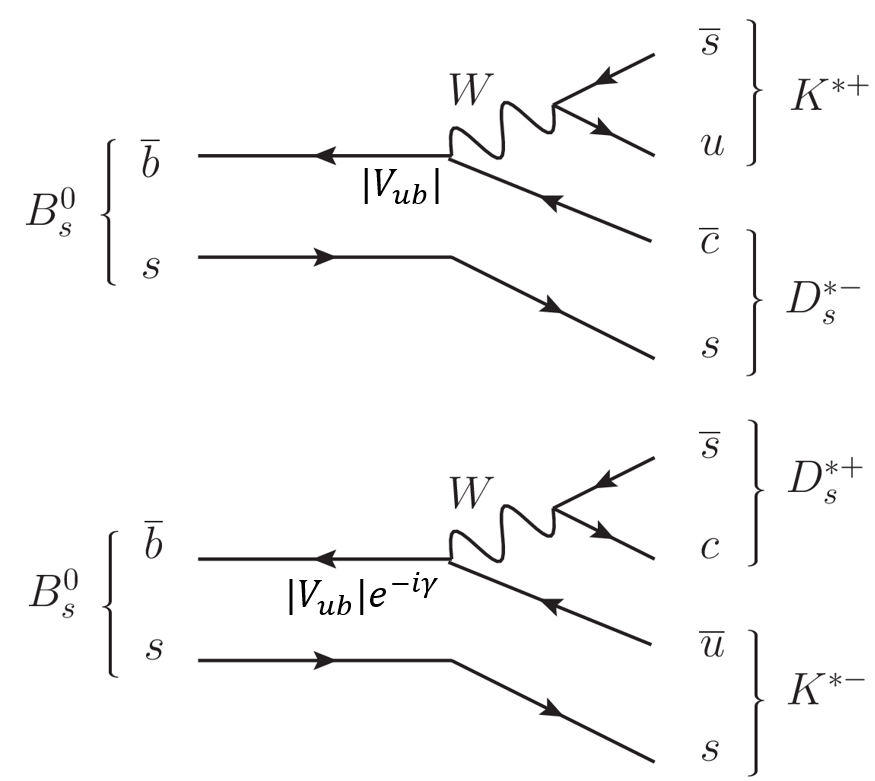
\includegraphics[width=9cm]{figs/feynman_diagram.png}
\centering
\caption{Feynman diagram for \Bs\to\Dss\Kstarm decay. }
\label{fig:feymnan}
\end{figure}


\clearpage
\clearpage
\section{Analysis strategy}\label{analysis_strategy}

This section presents an analysis strategy for branching fraction calculation of  \Bs~\to\Dss\KS\pim and \Bs~\to\Dss\Kstarm decays and analysis of reference channel XX . It is organised as follows: Chapter \ref{sec::data_sample} describe data sample, stripping selection, trigger lines used in this analysis and simulated samples. Chapter \ref{sec::selection} describes preliminary selection \Ds, \KS, and\Dstar, multivariate analysis using BDT and post-MVA selection. 
\section{Data Samples}\label{sec::data_sample}

This analysis is based on a data sample over \lhcb Runs  2, collected between 2015-2018. The total integrated luminosity for \lhcb during this time is approximately 6.0\invfb. Data is taken from different stripping lines for different years (Tab.\ref{tab:strippings}).\\

\begin{table}[ht]
    \centering
    \begin{tabular}{c|c|c|c}
        Year & Stripping Used & Integrated luminosity (\invfb) & Energy (TeV) \\
        \hline\hline
        2015 & \texttt{Stripping24r1} & 0.328 & 6.5\\
        2016 & \texttt{Stripping28r1} & 1.665 & 6.5\\
        2017 & \texttt{Stripping29r2} & 1.609 & 6.5\\
        2018 & \texttt{Stripping34} & X.XX & 6.5\\
    \end{tabular}
    \caption{Summary of the data used in the analysis, where \sqs represents the center of the mass-energy of the proton-proton collisions}
    \label{tab:strippings}
\end{table}

Data is taken from \texttt{B02DsstKsPiLLDsst2DGammaD2HHHBeauty2CharmLine} and \texttt{B02DsstKsPiDDDsst2DGammaD2HHHBeauty2CharmLine} line in the BHADRON stripping stream which produce two sets of candidates, one set of LL candidates and one set of DD candidates. Below, in the Tab.\ref{tab:stripp_1}-Tab.\ref{tab:stripp_10} there are listed detailes of stripping selection.

\vspace{1ex}
\begin{table}[h!]
\centering
\begin{tabular}{|c|c|} \hline
\multicolumn{2}{|c|}{\bf{KS0DDDInputsBeauty2CharmFilter}}\\ \hline
PT & $\ > 250$ MeV \\ \hline
M & $ \in (467,527)\ $MeV \\ \hline
\end{tabular}
\caption{\KS downstream stripping selection.}
\label{tab:stripp_1}
\end{table}

\vspace{1ex}
\begin{table}[h!]
\centering
\begin{tabular}{|c|c|} \hline
\multicolumn{2}{|c|}{\bf{PiInputsBeauty2CharmFilter}}\\ \hline
Track $\chi^2$ & $\ < 4$ \\ \hline
PT & $ > 100\ $MeV \\ \hline
P & $ > 1000 \ $MeV \\ \hline
Min. IP & $ > 4$ \\ \hline
TRGHP & $ < 0.4$ \\ \hline
\end{tabular}
\caption{\pion from \Ds stripping selection.}
\end{table}


\vspace{1ex}
\begin{table}[h!]
\centering
\begin{tabular}{|c|c|} \hline
\multicolumn{2}{|c|}{\bf{PiPIDTopoInputsBeauty2CharmFilter}}\\ \hline
PT & $ > 500\ $MeV \\ \hline
P & $ > 5000 \ $MeV \\ \hline
\multicolumn{2}{|c|}{\bf{PiPIDInputsBeauty2CharmFilter}}\\ \hline
PIDK & $ < 20$ \\ \hline
\end{tabular}
\caption{Additional \pion stripping selection.}
\label{tab:stripp_3}
\end{table}

\vspace{1ex}
\begin{table}[h!]
\centering
\begin{tabular}{|c|c|} \hline
\multicolumn{2}{|c|}{\bf{GammaBeauty2CharmFilter}}\\ \hline
PT & $\ > 90$ MeV \\ \hline
CL & $\ > 0.25$ \\ \hline
\end{tabular}
\caption{\g stripping selection.}
\label{tab:stripp_4}
\end{table}


\vspace{1ex}
\begin{table}[h!]
\centering
\begin{tabular}{|c|c|} \hline
\multicolumn{2}{|c|}{\bf{PiInputsBeauty2CharmFilter}}\\ \hline
$\chi^2$ śladu & $\ < 4$ \\ \hline
PT & $ > 100\ $MeV \\ \hline
P & $ > 1000 \ $MeV \\ \hline
Min. IP & $ > 4$ \\ \hline
TRGHP & $ < 0.4$ \\ \hline
\end{tabular}
\begin{tabular}{|c|c|} \hline
\multicolumn{2}{|c|}{\bf{KInputsBeauty2CharmFilter}}\\ \hline
$\chi^2$ śladu & $\ < 4$ \\ \hline
PT & $ > 100\ $MeV \\ \hline
P & $ > 1000 \ $MeV \\ \hline
Min. IP & $ > 4$ mm \\ \hline
TRGHP & $ < 0.4$ \\ \hline
\end{tabular}
\paragraph{}
\begin{tabular}{|c|c|} \hline
\multicolumn{2}{|c|}{\bf{D2HHHPIDBeauty2CharmFilter}}\\ \hline
Liczba $\pi$: PIDp $\ < 10$ & = 0 \\ \hline
Liczba $\pi$: PIDK $\ > 20$ & = 0 \\ \hline
Liczba $K$: PIDK $\ < -10$ & = 0 \\ \hline
\end{tabular}
\caption{\pion and \kaon from \Ds stripping selection.}
\label{tab:stripp_6}
\end{table}


\vspace{1ex}
\begin{table}[h!]
\centering
\begin{tabular}{|c|c|} \hline
\multicolumn{2}{|c|}{\bf{Dsst2DGammaCPVD2HHHBeauty2Charm}}\\ \hline
$|\Delta_M|$ & $\in (80,250)$ MeV \\ \hline
\end{tabular}
\caption{\Dss stripping selection.}
\label{tab:stripp_7}
\end{table}

\vspace{1ex}
\begin{table}[h!]
\centering
\begin{tabular}{|c|c|} \hline
\multicolumn{2}{|c|}{\bf{B02DsstKsPiDDDsst2DGammaD2HHHBeauty2Charm}}\\ \hline
$\chi^2$ śladu & $ < 4 \ $ \\ \hline
DIRA & $ > \ 0.999$ \\ \hline
$\tau$  & $ > \ 0.2 \ $ps \\ \hline
IP $\chi^2$ & $<25$ \\ \hline
PT & $ > 500\ $MeV \\ \hline
P & $ > 5000 \ $MeV \\ \hline
BPVVDCHI2 & $ > 1000$ \\ \hline
VFASPF(VCHI2/VDOF) & $ < 10$ \\ \hline
\end{tabular}
\caption{\Bs stripping selection.}
\label{tab:stripp_8}
\end{table}

\vspace{1ex}
\begin{table}[h!]
\centering
\begin{tabular}{|c|c|} \hline
\multicolumn{2}{|c|}{\bf{First \Bs daughter}}\\ \hline
P & $ > 10000\ $MeV \\ \hline
PT & $ > 1700 \ $MeV \\ \hline
$\chi^2$ śladu & $ < 4 \ $ \\ \hline
Min. IP & $ < 16 \ $ \\ \hline
Min. IP PV & $ > 0.1 \ $mm \\ \hline
\end{tabular}
\caption{\Bs daughter stripping selection.}
\label{tab:stripp_9}
\end{table}

\vspace{1ex}
\begin{table}[h!]
\centering
\begin{tabular}{|c|c|} \hline
\multicolumn{2}{|c|}{\bf{Second \Bs daughter}}\\ \hline
\ \ \ $\chi^2$ \ śladu \ \ \ & $ < 4 \ $ \\ \hline
PT & $ > 500 \ \ $MeV \\ \hline
P & $ > 5000 \ $MeV \\ \hline
\multicolumn{2}{|c|}{\bf{or}}\\ \hline
ID & $K_s^0 \ $ \\ \hline
PT & $ > 500 \ $MeV \\ \hline
\ \ \ \ P \ \ \ \ \ & $ > 5000 \ $MeV \\ \hline
\end{tabular}
\caption{\Bs daughter stripping selection.}
\label{tab:stripp_10}
\end{table}

The additional requirement was made in \Bs\to\Dss\Kstarm analysis. Since there is no stripping selection for the \Kstarm the preselection of \Kstar base on the cut on invariant mass of \KS\pim: $m(\KS\pim)< 1400$ MeV.  The Fig. \ref{fig:kstar_stripp} present invariant mass of \KS\pim candidates after $m(\KS\pim)< 1400$ MeV for 2015 data sample. The red colour indicates 75 MeV mass windows around the nominal mass of \Kstarm. Only events with \Kstarm mass within this mass window will be considered in the Bs\to\Dss\Kstarm analysis. 

\begin{figure}[h]
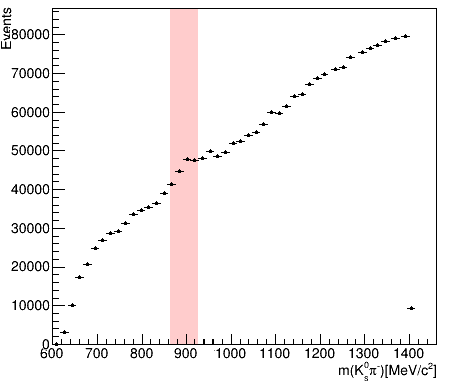
\includegraphics[width=9cm]{figs/introduction/Kstar_stripping.png}
\centering
\caption{Invariant mass of \KS\pim candidates for 2015 data sample with $m(\KS\pim)< 1400$ MeV cut. The red color indicate 75 MeV mass windows around nominal mass of \Kstarm(892)}
\label{fig:kstar_stripp}
\end{figure}



\subsection{Trigger}

All  candidates used in this analysis are required to have passed the following triggers:

\begin{itemize}
    \item \texttt{L0HadronDecision}
    \item \texttt{L0MuonDecision}
    \item \texttt{L0DiMuonDecision}
    \item \texttt{L0ElectronDecision}
    \item \texttt{L0PhotonDecision}
    \item \texttt{Hlt1TrackMVADecision}
    \item \texttt{Hlt1TwoTrackMVADecision}
    \item \texttt{Hlt2IncPhiDecision}
    \item \texttt{Hlt2Topo2BodyDecision}
    \item \texttt{Hlt2Topo3BodyDecision}
    \item \texttt{Hlt2Topo4BodyDecision}
    
\end{itemize}

\subsection{Simulated events}

Several Monte Carlo simulated samples were used in several parts of this analysis. These samples have been divided due to the method of production.  MC is generated for both the signal mode and all considered background modes. 

\subsubsection{Full simulated events}

Full simulation samples have been generated for signal and background modes. Both magnet polarities were generated, the 2016 sample was generated with Pythia8 and Sim09, the 2020 sample was generates with PythiaX and SimX. All samples were generated with all daughters in LHCb acceptance. The signal sample is produced with the \Ds decay to  \Dsp~\to\Kp\Km\pip. The specific MC data samples requested may be found in Tab.\ref{tab:MC_Full}.

\begin{table}[ht]
    \centering
    \begin{tabular}{ccccc}
        \hline
        Event type number & Year &   Decay & Options & Type\\
        \hline
        13266301 & 2016 & \Bs\to\Dss\Kstarm & \texttt{sqDalitz, DecProdCut} & DST\\
        XXXXXXX & 2020 & \Bs\to\Dss\KS\pim & \texttt{sqDalitz, DecProdCut}\\
        XXXXXXX & 2020 & \Bs\to\Dp\KS\pim & \texttt{sqDalitz, DecProdCut}\\
        13264221  & 2018 & \Bs\to\Dss\pim & \texttt{sqDalitz, DecProdCut} & DST\\
        
    \end{tabular}
    \caption{Full MC samples used  in analysis}
    \label{tab:MC_Full}
\end{table}

\subsubsection{Simplify simulated events}

The simplify simulated events have been generated using RapidSim simulation package. RapidSim allows for the fast simulation of phase space decays of beauty and charm quark hadrons, allowing quick studies of the properties of signal and background decays in physics analysis. RapidSim features generations of events using different identification hypotheses, different range of momentum, and angular acceptance of the detector.  The specific MC data samples generated using RapidSim may be found in Tab.\ref{tab:MC_Simple}.


\begin{table}[ht]
    \centering
    \begin{tabular}{ccc}
        \hline
        Sample Number &  Decay & Options\\
        \hline
        1 &  XXXXXXX  & \texttt{option}\\
    \end{tabular}
    \caption{Simplify MC samples used in analysis}
    \label{tab:MC_Simple}
\end{table}

\subsubsection{MC application in MVA}

As the simulated events pass the stripping line condition, they represent the decay signal and can be used in training of multivariate analysis method. As the number of events useful in Multivariate Analysis' method training was low (what can result in overtraining the method ..... , *multiplication?*).

\subsubsection{MC application in efficiency calculation}

Another application of simulated events is a calculation of efficiency of both selection criteria and BDT method. Efficiency is calculated for each criterion as the number of MC events that pass the requirements to the total number of simulated events.  Since the expected number of data events is low, both efficiencies should be as big as possible. Selection efficiency is used in the calculation of total efficiency, which is taken into account during relative branching fraction calculation. 
\clearpage
\section{Offline Selection}\label{sec::selection}

The offline selection focuses on selecting intermediate states \Ds and \KS and resonance states \Dss and \Kstarm. Tables and summarize all selection requirements, which are described in the following paragraph.  Tables 3.1 and 3.2 summarize all selection requirements. The high number of proton-proton interactions during data talking resulted in a large fraction of events having more than one reconstructed PV. These events are called multiple events. There are no multiply events after all selection stages in this analysis, and we didn't perform the best candidates selection. More information can be found in section \ref{subsec::multi}. The preliminary selection of candidates is divided into a selection of each type of particle in the full decay chain. 

\subsection{Selection of \KS}

In LHCb \KS  mesons can be reconstructed using a different type of tracks. The type of track depends on detectors, which particle pass afters proton-proton collision in LHC. Long tracks are reconstructed from hits recorded in VELO, TT detector, and T stations. Downstream are a track of particle which did not pass VELO detector and are reconstructed only from TT and T stations hits. As a result, this particle's mass resolution is worse than for the long track, but the number of candidates is significantly bigger. The number and quality of candidates imply separate selection for long (LL) tracks and downstream (DD).

\begin{table}[h!]
\begin{center}
\begin{tabular}{ p{1cm}p{2cm}p{4.5cm}p{6cm} }
\hline
\hline
  & Variable  & Cut & Justification \\
 \hline
 DD   & $m(\pi\pi)$  & = $m_{\KS(PDG)} \pm$ 20 MeV & Selection genuine \KS\\ 
      & \KS $FD_{sig}$    & $> 7$ & Removing random combinations \\ 
 LL   & $m(\pi\pi)$  & = $m_{\KS(PDG)} \pm$ 20 MeV & Selection genuine \KS\\
 \hline
\end{tabular}
\caption{Offline selection requirements for \KS candidates.}
\label{tab:KS_sel}
\end{center}
\end{table}%

The $FD_{sig}$ stands for fight distance significance defind as:

\begin{equation}
    FD_{sig} = \frac{z_\KS - z_B}{\sqrt{\sigma^2_\KS-\sigma^2_B}}
\end{equation}

where $\sigma_\KS$ and $\sigma_B$  are the errors in the z position of the \KS and \B decay vertex. Flight distance significance is defined as the $z$ distance between the particle and \Bs end vertices divided by the sum in the quadrature of this position's uncertainties. The same requirement is also made for \Ds mesons to separate prompt \Ds mesons created in proton-proton collisions from that one from \B mesons decays. 

The efficiency of selection criteria is calculated using simulated events. Table \ref{tab:KS_eff} show efficiency of each selection requirement for \KS candidates.

\begin{table}[h!]
\begin{center}
\begin{tabular}{ p{1cm}p{2cm}p{4.5cm}p{6cm} }
\hline
\hline
  & Variable  & Cut & Signal Efficiency (\%) \\
 \hline
 DD   & $m(\pi\pi)$  & = $m_{\KS(PDG)} \pm $ 20 MeV & 96.6 \\ 
      & \KS $FD_{sig}$    & $> 7$ & 92.7 \\ 
 LL   & $m(\pi\pi)$  & = $m_{\KS(PDG)} \pm$ 20 MeV & 96.3 \\

 \hline
\end{tabular}
\caption{Efficiency of cuts  (\KS candidates).}
\label{tab:KS_eff}
\end{center}
\end{table}%

\subsection{Selection of \Ds}

The \Ds meson can be reconstructed using 3 decay modes: \Ds\to\Kp\Km\pip, \Ds\to\Kp\pim\pip and \Ds\to\pip\pim\pip since the branching fraction for \Ds\to\Kp\Km\pip is around 5 - 10 times bigger than for \Kp\pim\pip and \pip\pim\pip combination respectively only \Kp\Km\pip combination is considered in this analysis.

\begin{table}[h!]
\centering
\begin{tabular}{ p{4cm}p{4cm} }
\hline
\hline
  Mode & BR \\
 \hline
     \Ds\to\Kp\Km\pip    & (5.45 $\pm$ 0.17) \%  \\
     \Ds\to\Kp\pim\pip    & (0.66 $\pm$ 0.04) \%   \\
     \Ds\to\pip\pim\pip    & (1.09 $\pm$ 0.05) \%   \\
 \hline
\end{tabular}
\caption{Branching fraction of \Ds meson decay to 3$h$ final states}
\label{tab:Ds_br}
\end{table}%

Following requirements was made to remove the combinatorial background from misidentifying of kaons or pions and physical background from misidentification of \Dp or \Lc meson or a random combination of \kaon or \pion with \Dz. This combination can mimic signal final state.

\begin{enumerate}
   \item \Dp\to\Kp\pip\pim \\ 
   Misidentification of kaon from \Ds\to\Kp\Km\pip with \Dp\to\Kp\pim\pip. Removed if the mass of combination under \pion hypothesis is within \Dp $\pm$ 20 MeV mass window unless the combination under \kaon hypothesis is within \Ds $\pm$ 20 MeV mass window and kaon fulfill the stronger requirement of PIDK(\kaon).
   
   \item \Dz\to\Kp\pim or \Dz\to\Kp\Km \\ 
    Combination of \Dz\to\Kp\Km or \Dz\to\Kp\Km meson with random \Kp or \pip. removed if a combination of \Kp\pim or \Kp\Km  $>$ 1850. 
    
   \item \Lc\to\Kp\proton\pim \\ 
   Misidentification of kaon from \Ds\to\Kp\Km\pip with \Lc\to\Kp\proton\pip. Removed if the mass of combination under \proton hypothesis is within \Lc $\pm$ 20 MeV window unless the combination under \kaon hypothesis is within \Ds $\pm$ 20 MeV mass window and kaon fulfill the stronger requirement of PIDK(\kaon).
 \end{enumerate}
 
 
\begin{figure}[h!]
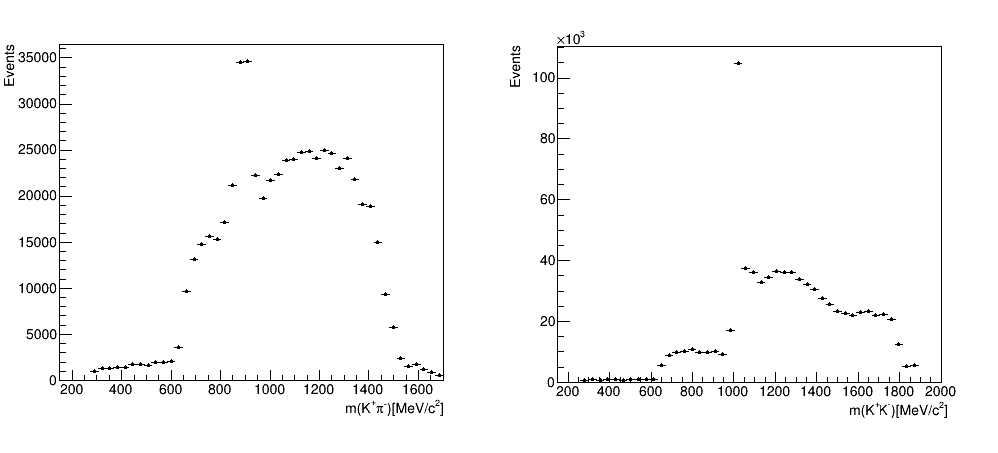
\includegraphics[width=14cm]{figs/Selection/reso.png}
\centering
\caption{Mass distribution of \Kp\Km (left) and \Kp\pim (right) candidates from \Ds\to\Kp\Km\pim (the 2015 data sample).}
\label{fig:reso}
\end{figure}

The Fig. \ref{fig:reso} show contributions from \Lc decay where the \proton is misidentified as \kaon , contributions from \Dz decay where the \pion is misidentified as \kaon, \kaon\pion and \kaon\kaon mass distribution with visible background contribution of \Dz meson. All of them were removed by applying vetos. Histograms were created using the 2015 data sample. 

 Since the \Ds meson decay to the combination of kaons and pions, it can decay by intermediate state \Ds\to(\Pphi\to\Kp\Km)\pip,  \Ds\to \Kp(\Kstarz\to\Km\pip) or by no-resonance mode to \Kp\pim\pip final state. \Pphi and \Kstarz has been investigated, but no additional requirements were made (Fig. \ref{fig:reso}). 

\begin{figure}[h!]
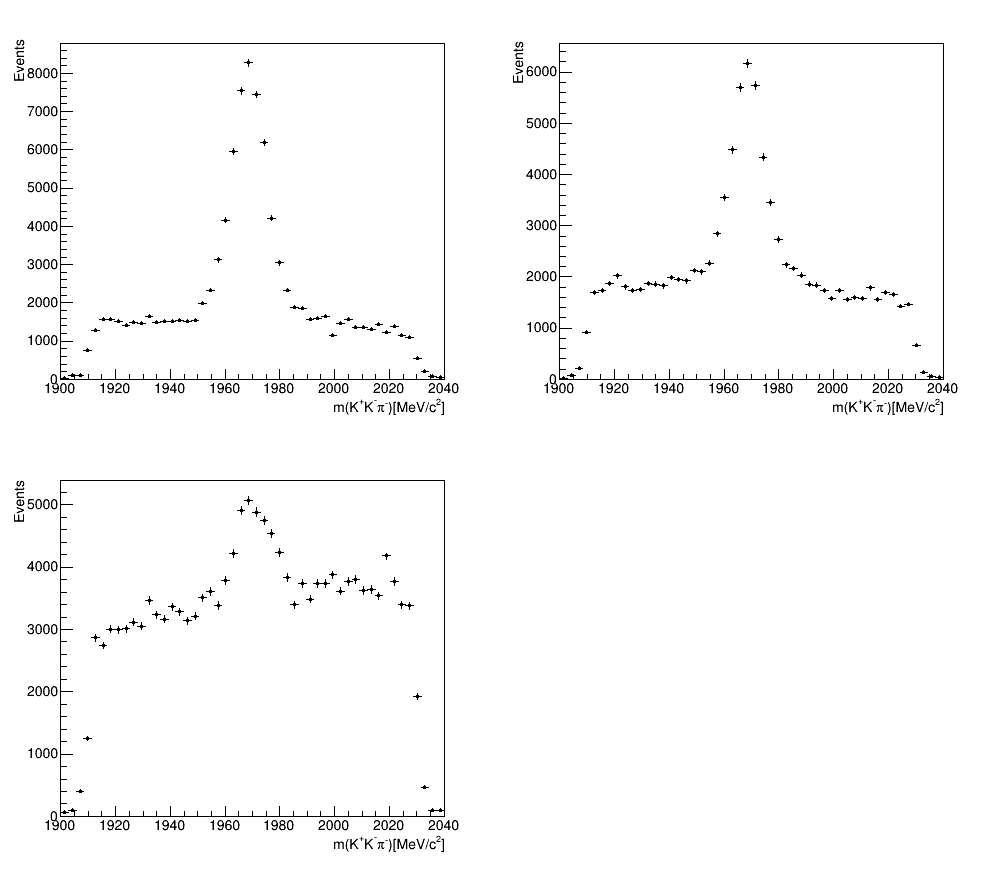
\includegraphics[width=14cm]{figs/Selection/D_reso.png}
\centering
\caption{Mass distribution \Ds\to(\Pphi\to\Kp\Km)\pip (left), \Ds\to \Kp(\Kstarz\to\Km\pip) (right) and no-resonance \Kp\pim\pip candidates mass distribution (bottom, the 2015 data sample).}
\label{fig:D_reso}
\end{figure}
 
The Fig. \ref{fig:D_reso} show \Ds\to(\Pphi\to\Kp\Km)\pip (left), \Ds\to \Kp(\Kstarz\to\Km\pip) (right) and no-resonance \Kp\pim\pip (bottom) candidates mass distribution. Visible is difference between signal to background ratio for each distribution. 

\begin{figure}[h]
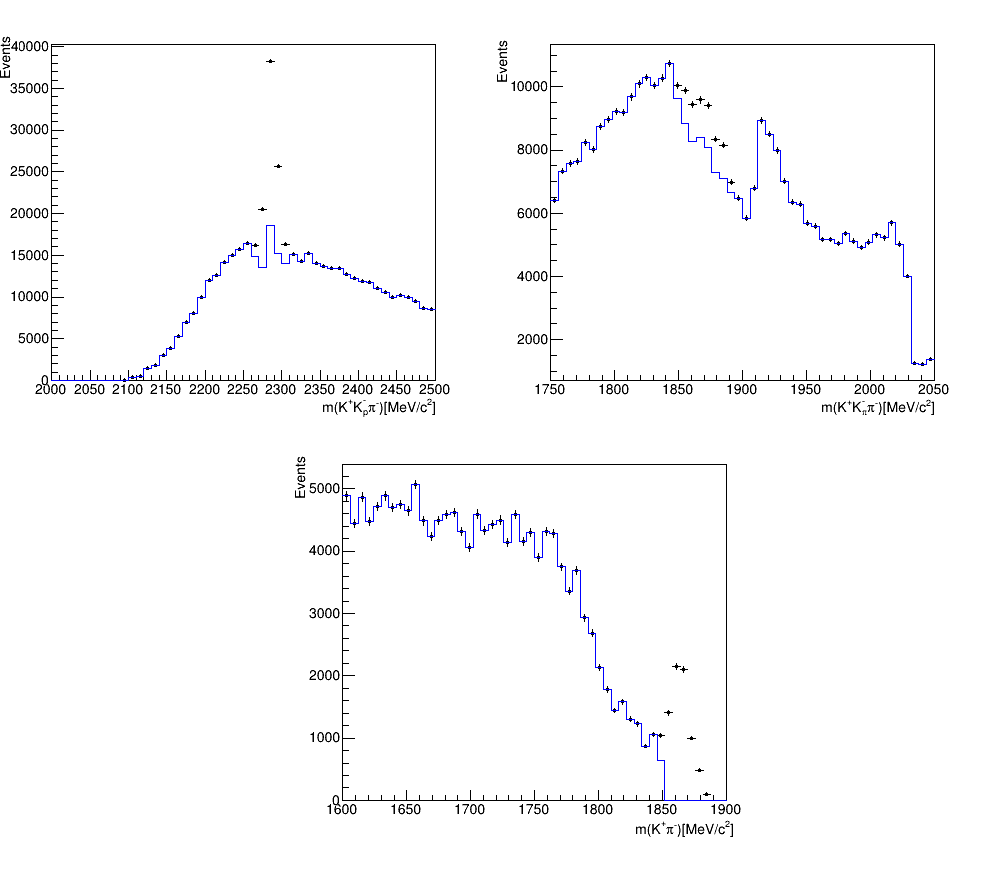
\includegraphics[width=14cm]{figs/Selection/Ds_vetos.png}
\centering
\caption{Background contributions from \Lc decay where the \proton is misidentified as \kaon The \Ds invariant mass is recalculated under proton mass hypothesis for the kaon, black dots are the mass distribution of \Kp\proton\pip before removing \Lc contribution, blue line - after (top left). Background contributions from \Dz decay where the \pion is misidentified as \kaon The \Ds invariant mass is recalculated under pion mass hypothesis for the kaon, black dots are the mass distribution of \Kp\pim\pip before removing \Dz contribution, blue line - after (top right). \kaon\pion and \kaon\kaon mass distribution with visible background contributions from \Dz meson before (black dots) and after (blue line) removing \Dz meson contribution (bottom).}
\label{fig:reso}
\end{figure}
 
 Since the \Dp meson contribution is removed by stripping, we do not expect \Dp mass peak to be visible on $\Kp\Km_{\pim}\pip$ mass distribution. 

\begin{figure}[h!]
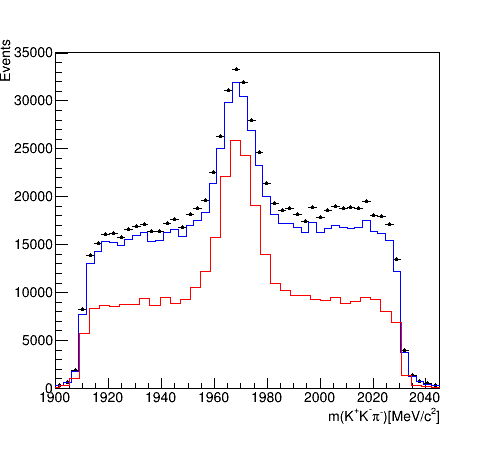
\includegraphics[width=10cm]{figs/Selection/D_mass.png}
\centering
\caption{The \Kp\Km\pip candidates mass distribution after stripping and PID cut (black dot), after applying vetos (blue line), after stripping, PID cut, applying vetos and kinematic cuts (red line, the 2015 data sample). }

\label{fig:D_mass}
\end{figure}

\begin{table}[h!]
\centering
\begin{tabular}{ p{3cm}p{3cm}p{9.5cm}}
\hline
\hline
& Description  & Requirement  \\
\hline
 \Ds\to\Kp\Km\pip   & $m(\Kp\Km\pip)$ & = $m_{\Ds}\pm$ 25 MeV \\ 
                    & PIDK(\kaon)     &   $>$ 5 \\
                    & PIDK(\pion)     &   $<$ 5 \\
                    & hasRich(\kaon / \pion) &    =  1 \\
                    & isMuon(\kaon / \pion) &     =  0 \\
                    & $FD_{sig}$ &     $>$ 0 \\
 & & \\
 \Dz veto   & $m(\Kp\Km)$  & $<$ 1850 MeV \\ 
            & $m(\Kp\pim)$ & $<$ 1850 MeV \\ 
 \Lc veto   & $m(\Kp\Km_{p}\pip)$  & $\neq m(\Lc) \pm 40 $ MeV $||$ PIDK(\Km) - PIDp(\Km) $>$ 5\\ 
 \Dp veto   & $m(\Kp\Km_{\pim}\pip)$  & $\neq m(\Dp) \pm 20 $ MeV $||$ PIDK(\Km) $>$ 7\\ 
 \hline
 \Ds\to\Kp\pim\pip   & $m(\Kp\pim\pip)$ & = $m_{\Ds}\pm$ 25 MeV \\ 
                    & PIDK(\kaon)     &   $>$ 5 \\
                    & PIDK(\pion)     &   $<$ 5 \\
                    & hasRich(\kaon / \pion) &    =  1 \\
                    & isMuon(\kaon / \pion) &     =  0 \\
                    & $FD_{sig}$ &     $>$ 0 \\
 & & \\
 \Dz veto   & $m(\Kp\pim)$ & $<$ 1850 MeV \\ 
 \hline
 \Ds\to\pip\pim\pip & $m(\pip\pim\pip)$ & = $m_{\Ds}\pm$ 25 MeV \\ 
                    & PIDK(\pion)     &   $<$ 0 \\
                    & hasRich(\kaon / \pion) &    =  1 \\
                    & isMuon(\kaon / \pion) &     =  0 \\
                    & $FD_{sig}$ &     $>$ 0 \\
\end{tabular}
\caption{Offline selection requirements for \Ds candidates.}
\label{tab:Ds_sel}
\end{table}%

The efficiency of selection criteria was calculated for kinematic cut of \Ds candidates (Tab. \ref{tab:Ds_eff}).
 
\begin{table}[h!]
\centering
\begin{tabular}{p{3cm}p{4.5cm}p{6cm} }
\hline
\hline
 Variable  & Cut & Signal Efficiency (\%) \\
 \hline
  $m(\Kp\Km\pip)$  & = $m_{\Ds}\pm$ 25 MeV & 83.9 \\ 
  hasRich(\kaon / \pion)    &  =  1 & 99.1 \\ 
  isMuon(\kaon / \pion)  & =  0 & 96.3 \\
  \Ds $FD_{sig}$    &  $>$ 0 & 92.7  \\
 \hline
\end{tabular}
\caption{Efficiency of cuts (\Ds candidates).}
\label{tab:Ds_eff}
\end{table}%

\subsection{Selection of  and \Dss}

Following paragraph describe the selection of resonance states \Dss. The offline selection of  \Dss base on the selection of \Ds mesons and \g.  The selection of \g is done by BDT described in the following paragraph. For \Dss resonances, an additional requirement is made. The $\Delta_M$ variable describes the mass difference between \Dss and \Ds. The mass of the particle is well-known, and the difference of these masses should be around 144 MeV so, $\Delta_M$ requirement is $\Delta_M \in (104,184) $ MeV. 

\begin{table}[h!]
\begin{center}
\begin{tabular}{ p{3cm}p{3cm}p{5.5cm}}
\hline
\hline
& Description  & Requirement  \\
\hline
\Dss  & $\Delta_M $ & $\in (104,184)$ \\ 
\hline

\end{tabular}
\caption{Offline selection requirements for \Dss candidates.}
\label{tab:Reso_sel}
\end{center}
\end{table}%

 
\begin{table}[h!]
\centering
\begin{tabular}{p{3cm}p{4.5cm}p{6cm} }
\hline
\hline
 Variable  & Cut & Signal Efficiency (\%) \\
 \hline
  $\Delta_M $    & $\in (104,184)$  & 82.6 \\ 
 \hline
\end{tabular}
\caption{Efficiency of cuts (\Dss candidates).}
\label{tab:Reso_eff}
\end{table}%



\subsection{Multiple candidates selection}
\label{subsec::multi}

Reconstruction of events may result in more than one signal candidate for the same \Bs events. It is generally associated with a number of candidates for a photon and combinations of \Ds meson daughters. The multiplication factor was calculated after each stage of selection to ensure that at the end, no more than one candidate per event left. In the table Tab. \ref{tab:multi2015raw}-\ref{tab:multi2018sel} there are multiple candidates rate for stripping and preselected, Run 2 sample (Appendix \ref{app::A}). Since no more than 1 or 2 events with no more than 2 candidates per event left after all selection criteria (Tab. \ref{tab:multiBDT}), no additional action has been taken. 

\begin{table}[h!]
\begin{center}
\begin{tabular}{ p{2.6cm}p{3.1cm}p{0.6cm} }
\hline
\hline
Multip.  & Number of events & \% \\
\hline
    \multicolumn{3}{c}{Run Downstream}\\
\hline

     1    & 1638	& 99,9 \\
     2    & 2	& 0,01 \\

\hline
\end{tabular}
\quad
\begin{tabular}{ p{2.6cm}p{3.1cm}p{0.6cm} }
\hline
\hline
Multip.  & Number of events & \% \\
\hline
    \multicolumn{3}{c}{Run 2 Long}\\
\hline

     1    & 1195	& 99,9 \\
     2    & 2	& 0,01 \\

\hline
\end{tabular}
\caption{Multiple candidate rate for Run 2 data sample after selection.}
\label{tab:multiBDT}
\end{center}
\end{table}%

\subsection{Selection of \Kstarm (construction works)}
\label{subsex::veto_non_reso}

In the analysis of \Bs\to\Dssp\Kstarm the non-resonant background is reduced by removing events in which the \KS\pion invariant mass is greater than 75 MeV from the nominal \Kstarm mass. The \Bs\to\Dssp\Kstarm is a pseudoscalar to vector-vector, decay, which means the \Kstarm  must be londitudially polarised, so the \KS helicity angle  follows a $cos^2\theta$ distribution *** Removing events with an absolute value of $cos^2\theta$ less than 0.3 improves the


\begin{table}[h!]
\begin{center}
\begin{tabular}{ p{3cm}p{3cm}p{5.5cm}}
\hline
\hline
& Description  & Requirement  \\
\hline
\Kstar  &  PIDK(\pion)     &   $<$ 0 \\
\hline
\end{tabular}
\caption{Offline selection requirements for \Kstar candidates.}
\label{tab:Reso_kstar_sel}
\end{center}
\end{table}%

 
\begin{table}[h!]
\centering
\begin{tabular}{p{3cm}p{4.5cm}p{6cm} }
\hline
\hline
 Variable  & Cut & Signal Efficiency (\%) \\
 \hline
  PIDK(\pion)  & $<$ 0 & 86.6 \\ 
 \hline
\end{tabular}
\caption{Efficiency of cuts (\Kstar candidates).}
\label{tab:Reso_kstar_eff}
\end{table}%
\clearpage
\subsection{Boosted Decision Tree}

 Several MVA algorithms have been investigated, and a BDT algorithm with the gradient boost method using the  XGBoost framework \cite{XGBOOST} has been used to reduce the contribution of combinatorial background. The XGBoost library offers implementation of gradient boosting algorithms,
 
 Separate algoriths have been developed to reduce combinatorial background (\Bs BDT) and another to improve selection of \Kstarm(892) candidates (\Kstarm BDT). Since the downstream and long tracks have different properties, a separate algorithm was trained for both types of tracks. This apporach is applied for both algorithms: \Bs BDT and \Kstarm BDT.
 
\subsubsection{Configuration of the algorthm }

In order to reduce this dangerous over-fitting, some hyperparameters of the classifier
are adjusted:

\begin{itemize}
    \item \textit{learning rate - $\eta$} is used to prevents overfitting. $\eta$ 
    Learnig rate after each boosting step, shrinks the feature weights to make the boosting process more conservative.
    
    \item \textit{maximum depth} of a tree. Higher maximum depth make the model more complex and more likely to overfit. 
    
    \item \textit{minimum child weight} is a minimum sum of instance weight needed in a child. If the leaf node with the sum of instance weight is less than minimum child weight then the building process will give up further partitioning. 
    \item \textit{gamma} is a minimum loss reduction required to make a further partition on a leaf node of the tree. The larger gamma is, the more conservative the algorithm will be.
    
    \item \textit{subsample:} is a  ratio of the training sample. As a default is set to  0.5 what means that algorithm would randomly sample half of the training data prior to growing trees. and this will prevent overfitting. Subsampling will occur once in every boosting iteration.
    
\end{itemize}

The following parametrisation has been choosed in order to increase efficiency of algorithm:

\begin{table}[h!]
\begin{center}
\begin{tabular}{ p{3.6cm}p{3.1cm}}
\hline
\hline
Hyperparamter  &   Value \\
\hline
    learning rate    & 1638	\\
    maximum depth    & 1638	\\
    minimum child weighte    & 1638	\\
    gamma    & 1638	\\
    subsample    & 1638	\\
    
\hline
\caption{kk}
\end{tabular}
\end{center}
\end{table}

\subsubsection{Description of physics variables }

Besides a number of standard variables, a feature that estimates the imbalance of $p_T$ around the \Bs candidate momentum vector is also used. It is defined as

\begin{equation}
I_{p_T} = \frac{p_T(\Bs) - \sum p_T}{p_T(\Bs) + \sum p_T}
\label{eq::bdt_1}
\end{equation}

 where the sum is taken over all other charged tracks inconsistent with \Bs candidate. This cone is defined by a circle with a radius of 1.5 units in the plane of pseudorapidity and azimuthal angle (both defined below and expressed in radians). The $I_{p_T}$  enhance the selection of \Bs candidates.
 
 Another variables related to resonance states is $\Delta_R$:

\begin{equation}
\Delta_R(\Dsp) = \sqrt{(\eta(D_s)-\eta(\gamma))^2+(\phi(D_S)-\phi(\gamma))^2}
\label{eq::bdt_2}
\end{equation}
 
is also defined similarly for \Kstarm resonance, where $\eta$ and $\phi$ are the pseudorapidity and azimuthal angle in the LHCb lab. frame (the right-handed Cartesian system is being used, with the $z$ axis pointing along the beams direction). The polar angle - $\theta$, is measured with respect to the $z$ axis, the azimuthal angle - $\phi$, is the angle with respect to the $x$ axis of the projection in the $xy$ plane. The rapidity and pseudorapidity are defined as :

\begin{align} 
y = \frac{1}{2}ln(\frac{E+p_z}{E-p_z}) \\
\eta =- ln (tan \frac{\theta}{2})
\label{eq::bdt_3}
\end{align}

The $\Delta_R$ is known to be invariant under boost along the beams axis.  As the typical radius of a hadron jet in the $\eta-\phi$ plane has been measured to be about 1, expected value of $\Delta_R$ should be below 1.

The radial flight distance is defined as:

\begin{equation}
RFD(\Dsp) = \frac{Vx(\Dsp,z)-Vx(\Bs,z)}{\sigma_{Vx(\Dsp,z)}^2+\sigma_{Vx(\Bs,z)}^2}
\label{eq::bdt_4}
\end{equation}

where $\sigma_z$ stands for error in $z$ vertex position of particle. The $RFD$ variables is also used in selection of \KS mesons.
\subsubsection{Description of \Bs algorithm }

For \Bs BDT, a simulated sample was employed with generator level cuts and true matching applied. The background sample is data high mass sideband region of the \Bs mass (above 5600 MeV). For \Kstarm BDT, the same simulated sample with the same  true matching selection and \Kstarm low and high mass sideband region (belove 847 MeV and above 937 MeV).

\subsubsection{Description of \Kstar algorithm }


\subsubsection{\Bs algorithm}

Initial set of variables was investigated:

\begin{enumerate}

   \item \Dssp  and \Dssp daughters \\
    The $\Delta_R$ distance for \Dssp: $\Delta_R(\Dssp)$, the \Dsp impact parameter \chisq w.r.t PV: \Dsp IP\chisq, the \Dsp radial flight distance, RFD(\Dsp),  the \Dsp \chisq of the vertex: \Dsp Vx \chisq, the \g transverse momentum: \g $PT$, the \g condence level, \g CL, condence level is the probability that the Calo object tagged as a photon is indeed a photon. For true photons this variable peaks at 1, for fake photons - at 0.
    
   \item \Dsp daughters \\
   The ProbNN variables built using multivariate techniques by combining tracking and PID information from each sub-system into a single probability value for each particle hypothesis (kaon, pion, proton): \Kp, \Km ProbNNK and \pip ProbNNpi.
   %The transverse momenta:  \Kp, \Km, \pip $P_T$, the impact parameter \chisq w.r.t PV: \Kp, \Km, \pip IP\chisq, :
   
    \item \Bs meson \\
    The impact parameter \chisq w.r.t PV: \Bs IP\chisq, the $P_T$ asymmetry: $I_{p_T}$, the \chisqndf of the lifetime: \Bs $\tau$ \chisqndf, the \chisqndf of the end vertex: 
    \Bs Vx \chisq
  
\end{enumerate}

\begin{table}[h!]
\begin{center}
\begin{tabular}{ p{2cm}p{5cm} }
\hline
\hline
 Track type & Variable \\
 \hline
         & \Bs IP\chisq  \\
         & $I_{p_T}$ \\
         & \Bs $\tau$ \chisqndf \\
         & \Bs Vx \chisqndf  \\
         & \g $P_T$  \\
         & \g CL  \\
         & h1 ProbNNk  \\
         & h2 ProbNNk(pi)  \\
         & h3 ProbNNk(pi)  \\
         & $\Delta_R$ \Dss  \\
         & \Dsp IP\chisq  \\
         &  RFD(\Dsp)  \\
         & \Dsp Vx\chisq  \\
         & $\Delta_R$ \Dss  \\

\hline
\end{tabular}
\caption{BDT input variables}
\label{tab:BDT_var}
\end{center}
\end{table}%  

\subsubsection{\Kstarm algorithm}

Again, initial set of variables was investigated:

\begin{enumerate}

   \item \Kstarm  and \Kstarm daughters \\ 
   The $\Delta_R$ distance for \Kstarm: $\Delta_R(\Kstarm)$\\ 
   Classifier for long tracks: minimum and maximum impact parameter  \chisq w.r.t PV of \KS daughters: $\pip$, $\pim$ IP$\chisq_{max}$, IP$\chisq_{min}$, the \KS flight distance \chisq:  \KS FD\chisq, the \KS impact parameter \chisq w.r.t PV: \KS IP\chisq \\ 
   Classifier for downstream tracks: the \KS transverse momentum: \KS $P_T$ 


\end{enumerate}

\begin{table}
\begin{center}
\begin{tabular}{ p{2cm}p{5cm} }
\hline
\hline
 Track type & Variable \\
 \hline
         & $\Delta_R$ \Kstar  \\
         & \KS FD\chisq  \\
         & \\
        DD & \KS daughter 1 $P_T$  \\
        DD & \KS daughter 2 $P_T$  \\
         & \\
        LL & \KS daughter 1 IP$\chisq_{max}$  \\
        LL & \KS daughter 2 IP$\chisq_{max}$  \\
        LL & \KS daughter 1 IP$\chisq_{min}$  \\
        LL & \KS daughter 2 IP$\chisq_{min}$  \\        
        LL & \KS $\chi^2_{IP}$  \\

\hline
\end{tabular}
\caption{BDT input variables}
\label{tab:BDT_var}
\end{center}
\end{table}%   
   

\clearpage
\newpage
\section{MC and data comparison}

\begin{figure}[ht]
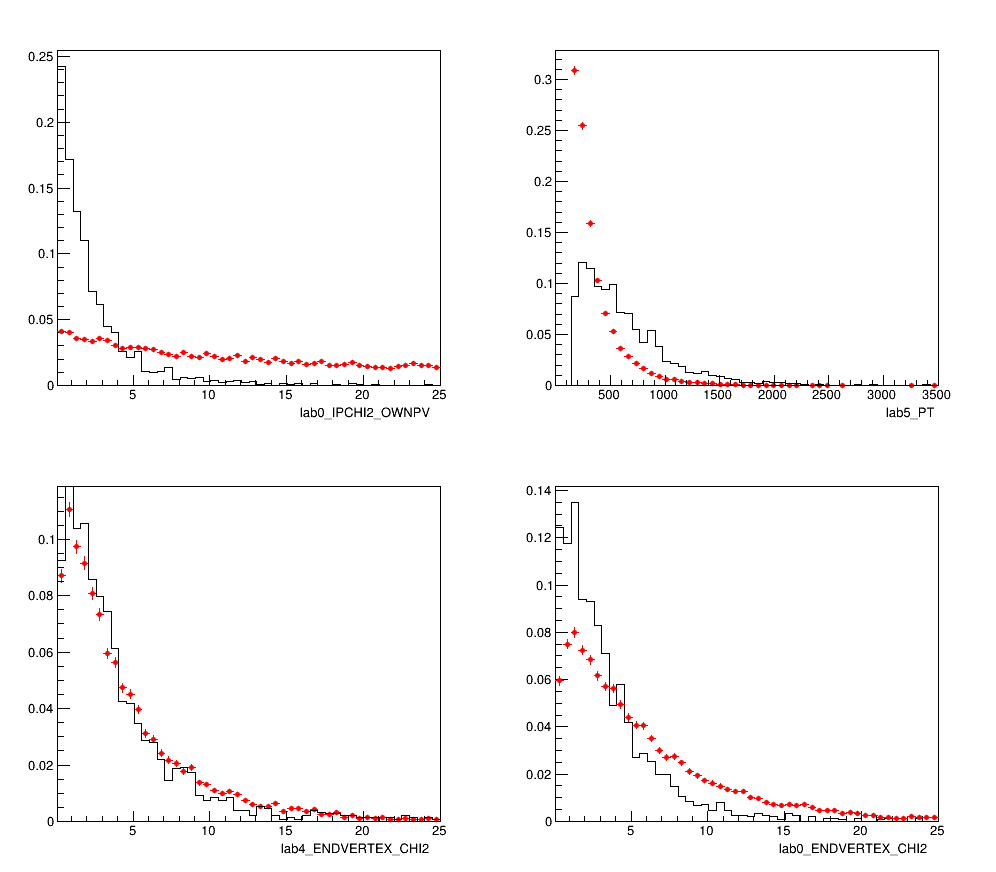
\includegraphics[width=11.5cm]{figs/MC_Data_Comp/DD0_0.png}
\centering
\caption{The comparison of simulated data (black lines) and Run 2 data (red dots) for selected variable, downstream tracks, data after preselection.}
\label{fig:MC_Data_Comp_DD0_0}
\end{figure}


\begin{figure}[hb]
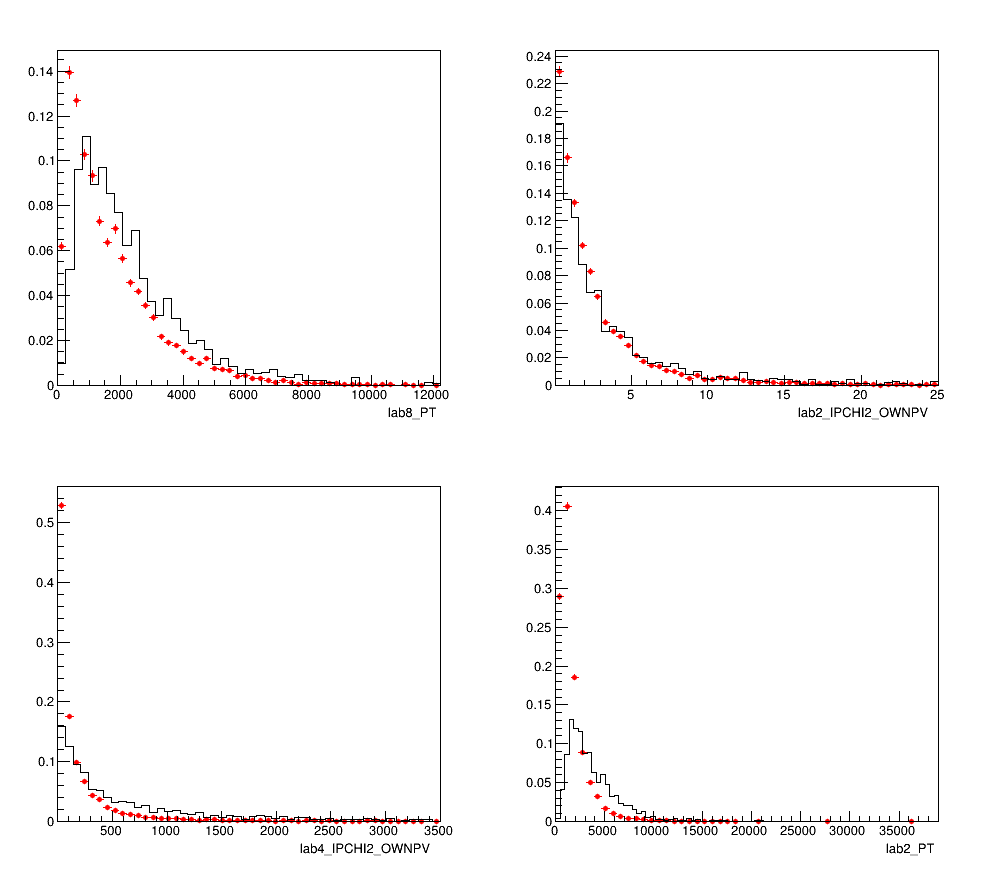
\includegraphics[width=11.5cm]{figs/MC_Data_Comp/DD0_1.png}
\centering
\caption{The comparison of simulated data (black lines) and Run 2 data (red dots) for selected variable, downstream tracks, data after preselection.}
\label{fig:MC_Data_Comp_DD0_1}
\end{figure}


\begin{figure}[ht]
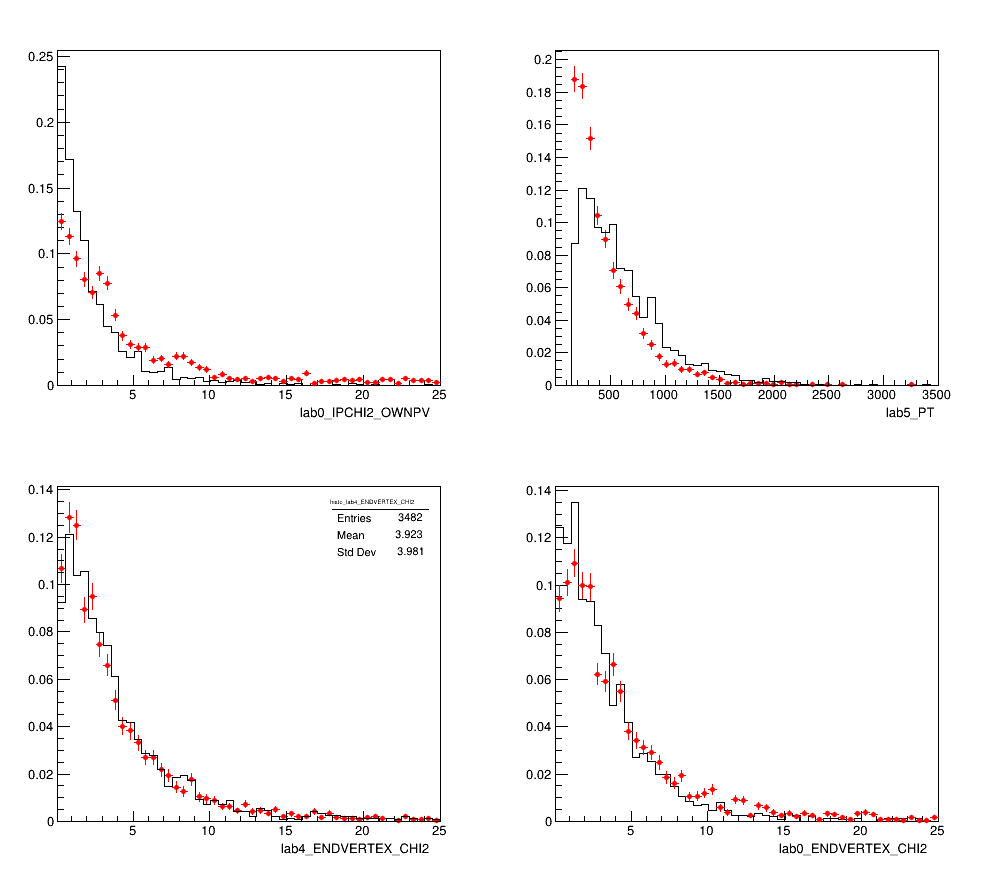
\includegraphics[width=11.5cm]{figs/MC_Data_Comp/DD1_0.png}
\centering
\caption{The comparison of simulated data (black lines) and Run 2 data (red dots) for selected variable, downstream tracks, data after preselection and BDT cut: BDT$>$0.1}
\label{fig:MC_Data_Comp_DD1_0}
\end{figure}


\begin{figure}[hb]
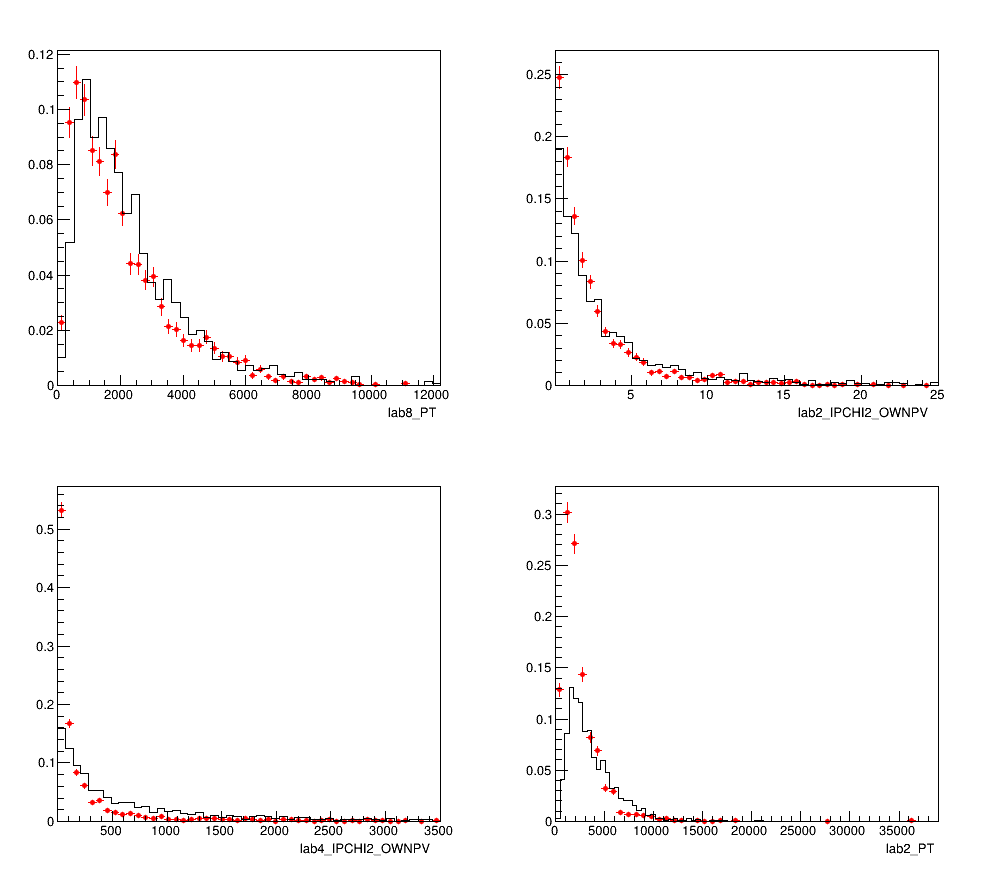
\includegraphics[width=11.8cm]{figs/MC_Data_Comp/DD1_1.png}
\centering
\caption{The comparison of simulated data (black lines) and Run 2 data (red dots) for selected variable, downstream tracks, data after preselection and BDT cut: BDT$>$0.1}
\label{fig:MC_Data_Comp_DD1_1}
\end{figure}


\begin{figure}[ht]
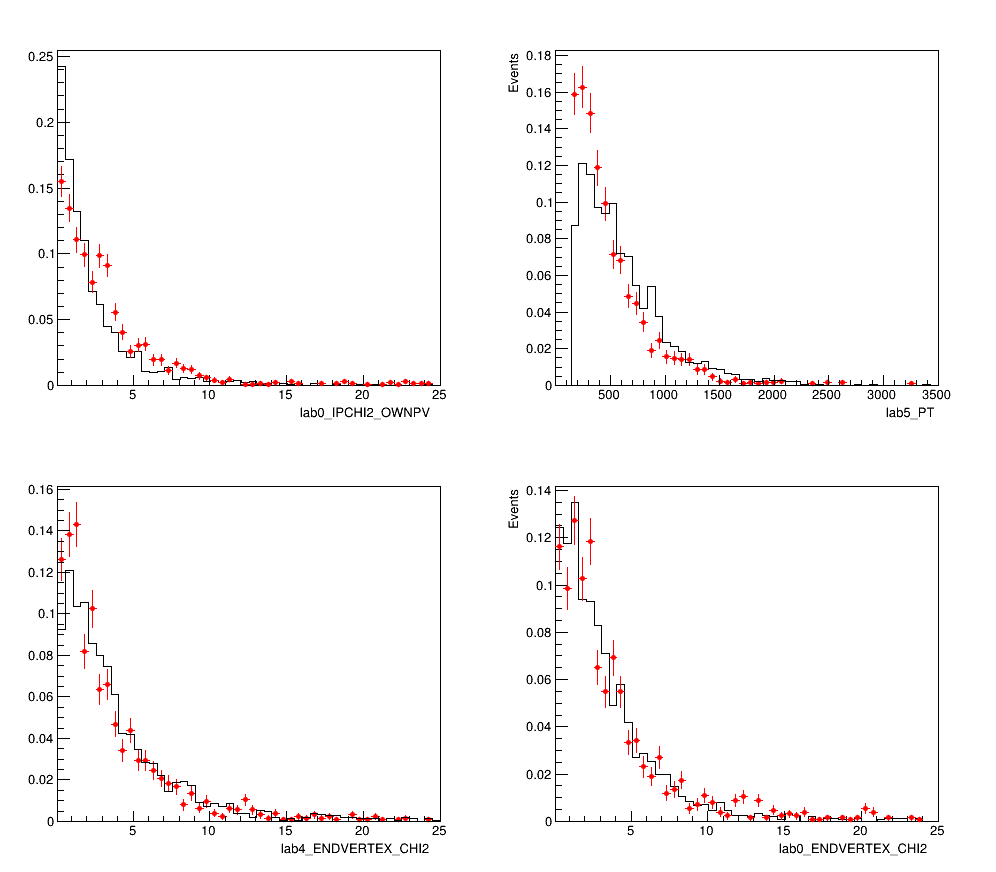
\includegraphics[width=11.5cm]{figs/MC_Data_Comp/DD8_0.png}
\centering
\caption{The comparison of simulated data (black lines) and Run 2 data (red dots) for selected variable, downstream tracks, data after preselection and BDT cut: BDT$>$0.8}
\label{fig:MC_Data_Comp_DD2_0}
\end{figure}


\begin{figure}[hb]
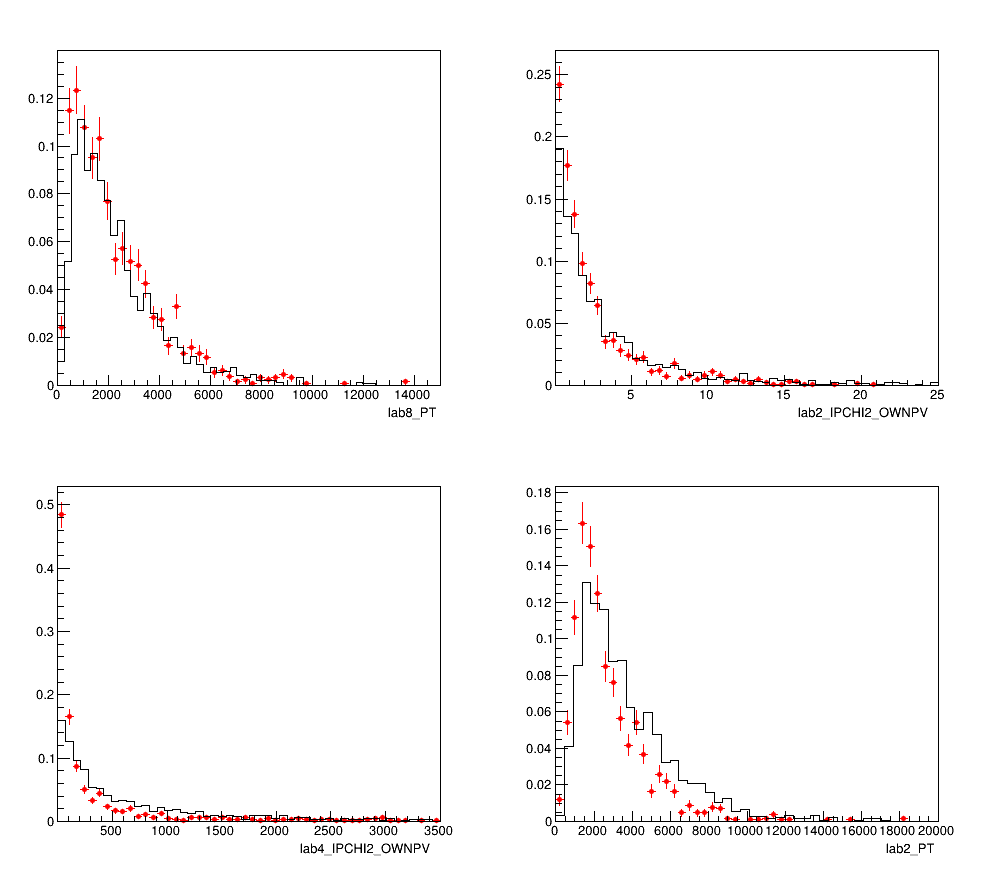
\includegraphics[width=11.5cm]{figs/MC_Data_Comp/DD8_1.png}
\centering
\caption{The comparison of simulated data (black lines) and Run 2 data (red dots) for selected variable, downstream tracks, data after preselection and BDT cut: BDT$>$0.8}
\label{fig:MC_Data_Comp_DD2_1}
\end{figure}


\begin{figure}[ht]
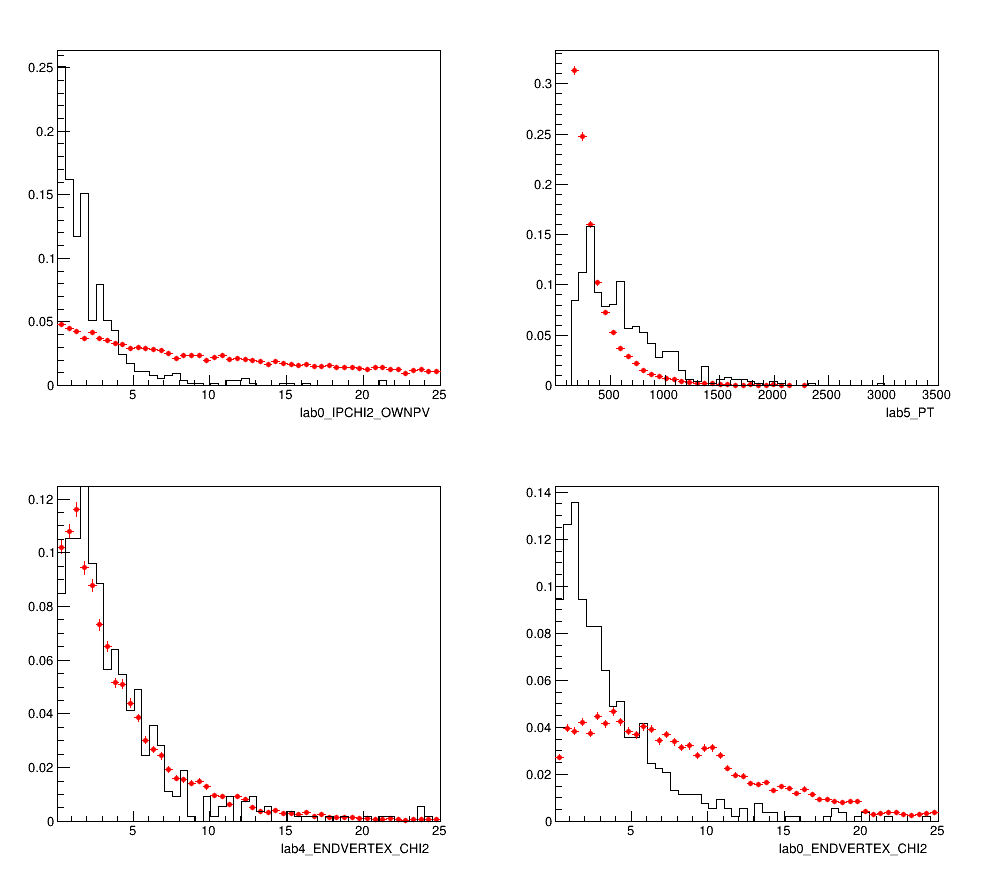
\includegraphics[width=11.5cm]{figs/MC_Data_Comp/LL0_0.png}
\centering
\caption{The comparison of simulated data (black lines) and Run 2 data (red dots) for selected variable, long tracks, data after preselection.}
\label{fig:MC_Data_Comp_LL0_0}
\end{figure}


\begin{figure}[hb]
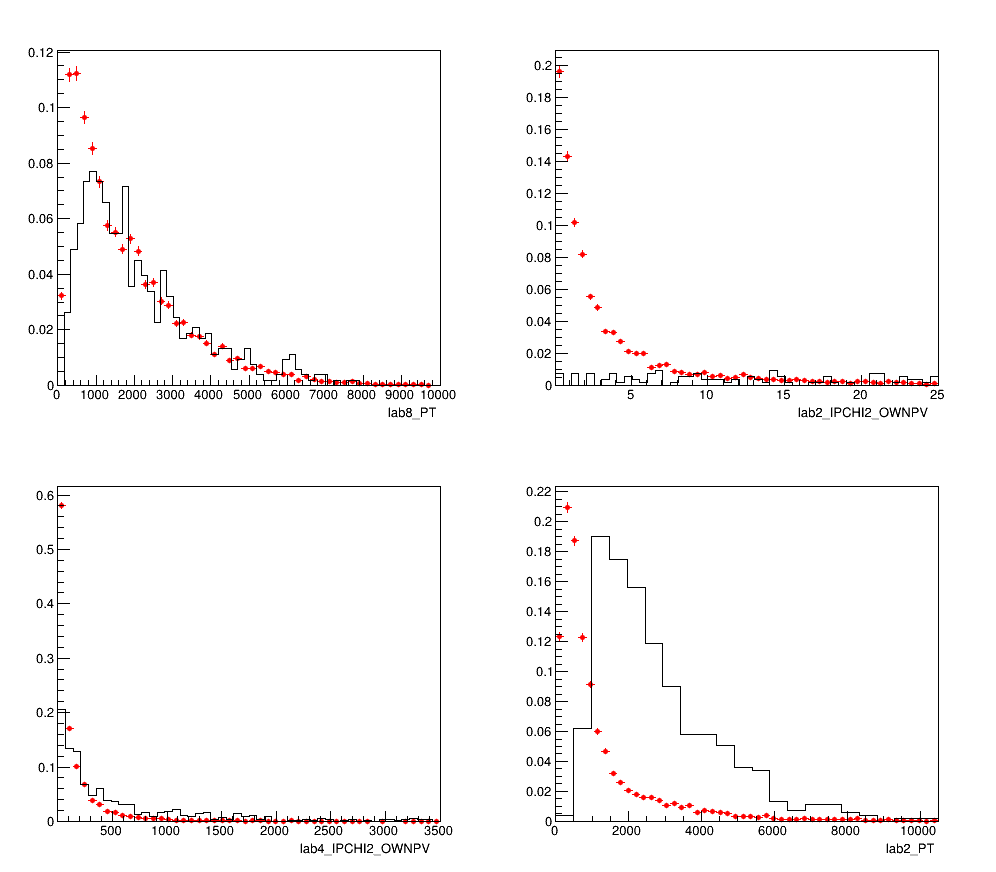
\includegraphics[width=11.5cm]{figs/MC_Data_Comp/LL0_1.png}
\centering
\caption{The comparison of simulated data (black lines) and Run 2 data (red dots) for selected variable, long tracks, data after preselection.}
\label{fig:MC_Data_Comp_LL0_1}
\end{figure}


\begin{figure}[ht]
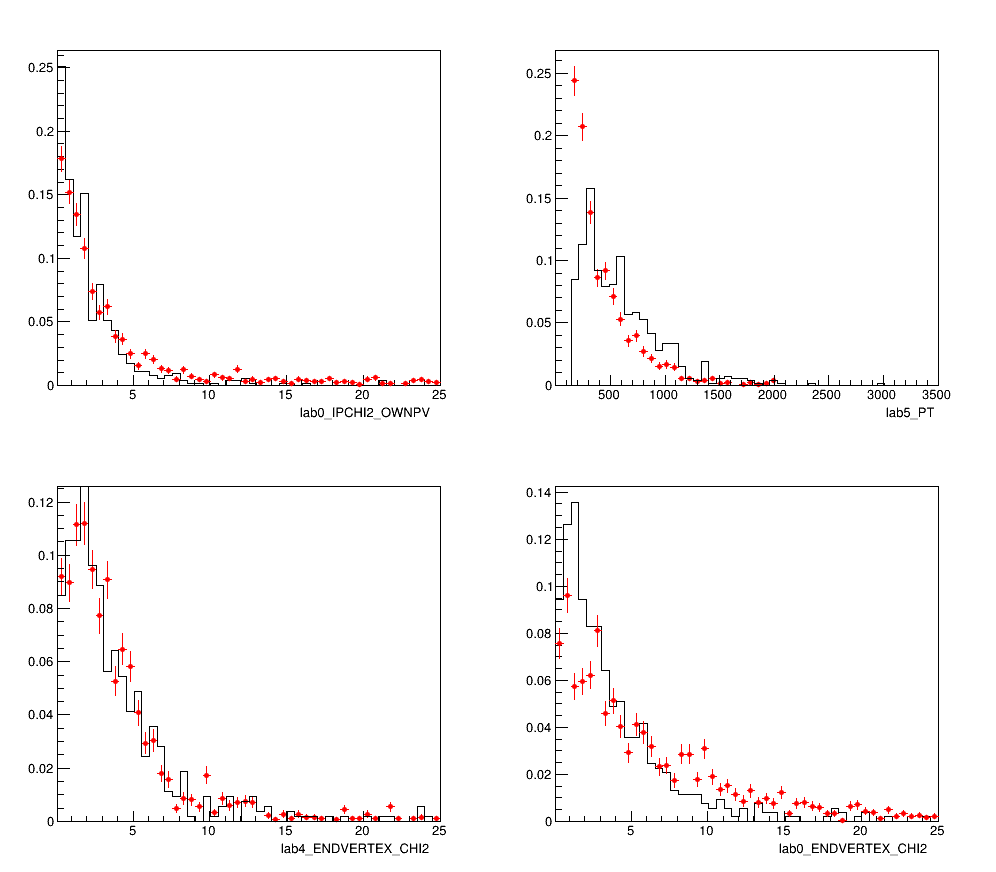
\includegraphics[width=11.5cm]{figs/MC_Data_Comp/LL1_0.png}
\centering
\caption{The comparison of simulated data (black lines) and Run 2 data (red dots) for selected variable, long tracks, data after preselection and BDT cut: BDT$>$0.1}
\label{fig:MC_Data_Comp_LL1_0}
\end{figure}


\begin{figure}[hb]
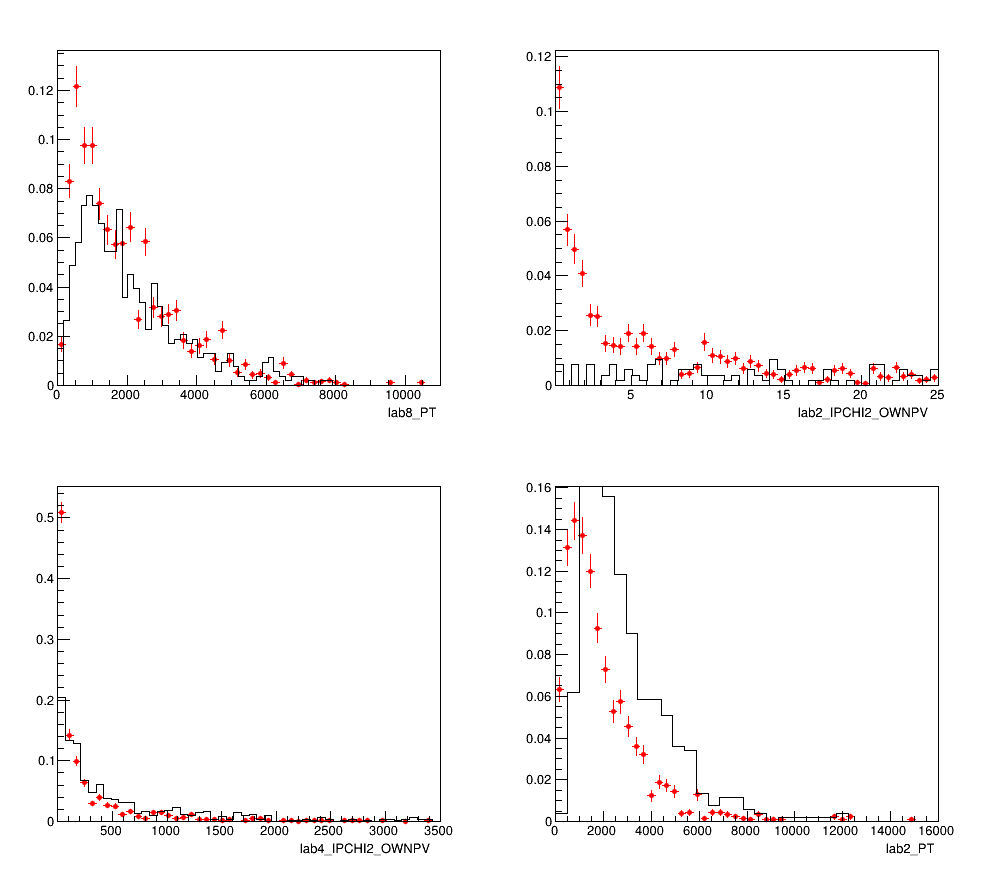
\includegraphics[width=11.5cm]{figs/MC_Data_Comp/LL1_1.png}
\centering
\caption{The comparison of simulated data (black lines) and Run 2 data (red dots) for selected variable, long tracks, data after preselection and BDT cut: BDT$>$0.1}
\label{fig:MC_Data_Comp_LL1_1}
\end{figure}


\begin{figure}[ht]
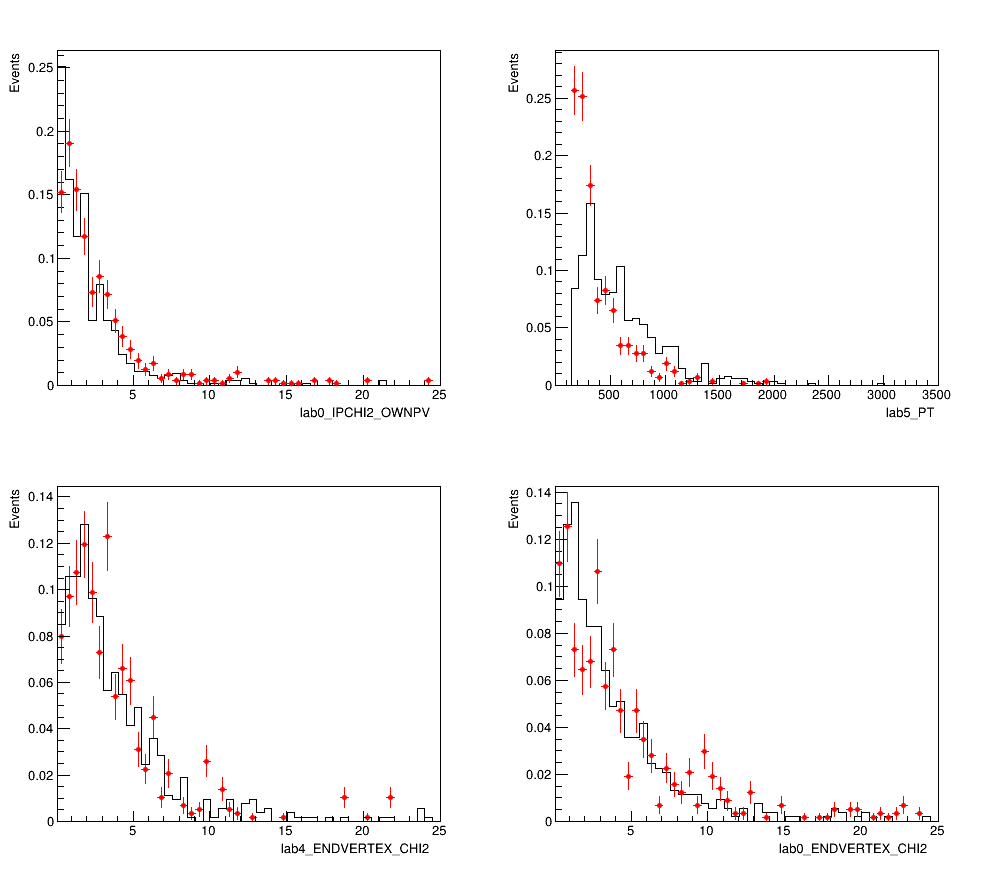
\includegraphics[width=11.5cm]{figs/MC_Data_Comp/LL8_0.png}
\centering
\caption{The comparison of simulated data (black lines) and Run 2 data (red dots) for selected variable, long tracks, data after preselection and BDT cut: BDT$>$0.8}
\label{fig:MC_Data_Comp_LL2_0}
\end{figure}


\begin{figure}[hb]
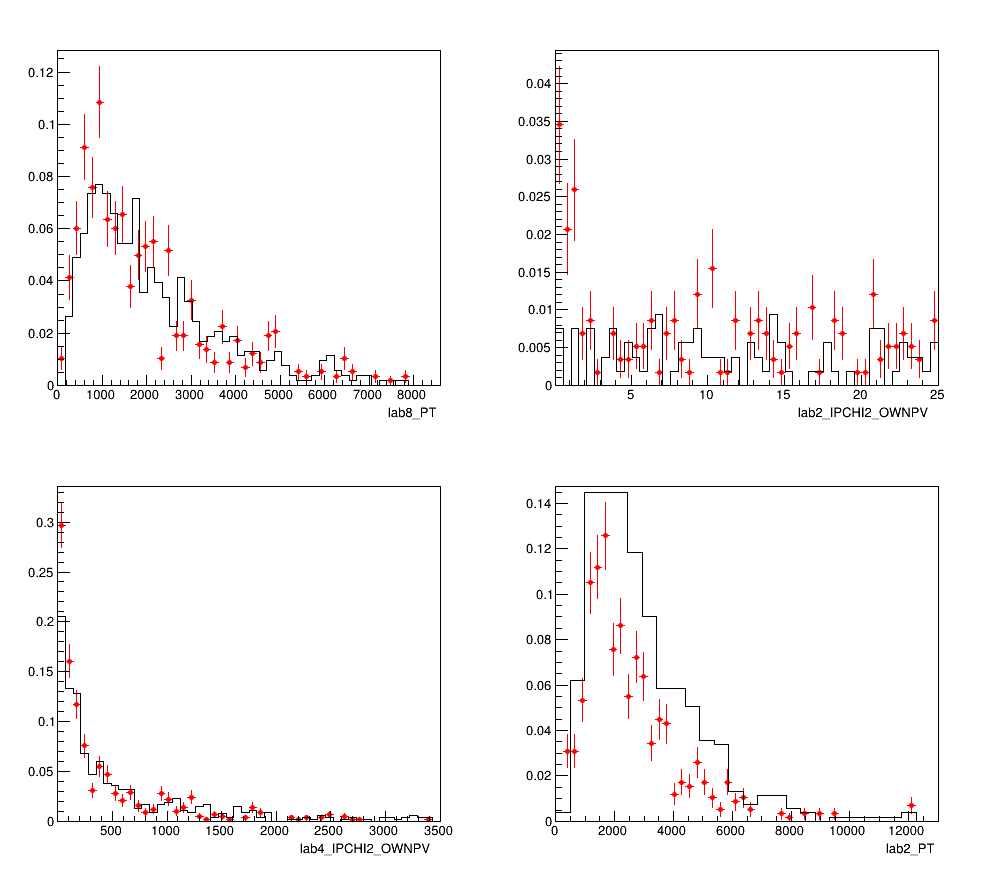
\includegraphics[width=11.5cm]{figs/MC_Data_Comp/LL8_1.png}
\centering
\caption{The comparison of simulated data (black lines) and Run 2 data (red dots) for selected variable, long tracks, data after preselection and BDT cut: BDT$>$0.8}
\label{fig:MC_Data_Comp_LL2_1}
\end{figure}

\newpage

\clearpage

%% Uncomment during review phase. 
%% Comment before a final submission.


% You can include short sections directly in the main tex file.
% However, for larger papers it is desirable to split the text into
% several semiautonomous files, which can be revised independently.
% This is especially useful when developing a document in
% collaboration with several people, since then different parts can be
% edited independently.  This type of file organization is shown here.
% 

%%%%%%%%%%%%%%%%%%%%%%%%%
%%%%% Appendixs %%%%%%%%%
%%%%%%%%%%%%%%%%%%%%%%%%%

\appendix
\section{Appendix A}
\label{app::A}
% the \\ the section title is centered below the phrase: AppendixA

\newpage
\newpage

Below, can be found summary of multiple candidates after stripping and preseletcion for 2015, 2016, 2017 and 2018.

\begin{table}[h!]
\begin{center}
\begin{tabular}{ p{2.6cm}p{3.1cm}p{0.6cm} }
\hline
\hline
Multip.  & Number of events & \% \\
\hline
    \multicolumn{3}{c}{2015 Downstream}\\
\hline
     1    & 436053 & 37,5 \\
     2    & 334000 & 28,7\\
     3    & 213991 & 18,4 \\
     4    & 213991 & 15,1 \\
     5    & 175635 & 9,1 \\
     6    & 106540 & 7,8 \\
     7    & 91041  & 4,3 \\
     8    & 50915  & 3,9 \\
    ...   &   ...  &  ... \\
    678   &    1 & -   \\
    1072  &    1 & -    \\
     
\hline
\end{tabular}
\quad
\begin{tabular}{ p{2.6cm}p{3.1cm}p{0.6cm} }
\hline
\hline
Multip.  & Number of events & \% \\
\hline
    \multicolumn{3}{c}{2015 Long}\\
\hline
     1    & 464700 & 26,7 \\
     2    & 353080 & 20,3\\
     3    & 228491 & 13,1 \\
     4    & 190532 & 11,0 \\
     5    & 116185 & 6.6 \\
     6    & 99605 & 5.7 \\
     7    & 57310  & 3,2\\
     8    & 51504 & 2,9\\
    ...   &   ...  &  ... \\
    732   &    1 & -   \\
    1020  &    1 & -    \\
     
\hline
\end{tabular}
\caption{Multiple candidate rate for 2015 stripping data.}
\label{tab:multi2015raw}
\end{center}
\end{table}%

\begin{table}[h!]
\begin{center}
\begin{tabular}{ p{2.6cm}p{3.1cm}p{0.6cm} }
\hline
\hline
Multip.  & Number of events & \% \\
\hline
    \multicolumn{3}{c}{2016 Downstream}\\
\hline
     1    & 3787227 & 27,5 \\
     2    & 2869520 & 20,9\\
     3    & 1835820 & 13,4 \\
     4    & 1490482 & 10,9 \\
     5    & 898392 & 6,5 \\
     6    & 757719 & 5,5 \\
     7    & 428491  & 3,1 \\
     8    & 380089  & 2,7 \\
    ...   &   ...  &  ... \\
    640   &    1 & -   \\
    735  &    1 & -    \\
     
\hline
\end{tabular}
\quad
\begin{tabular}{ p{2.6cm}p{3.1cm}p{0.6cm} }
\hline
\hline
Multip.  & Number of events & \% \\
\hline
    \multicolumn{3}{c}{2016 Long}\\
\hline
     1    & 464700 & 26,7 \\
     2    & 353080 & 20,3\\
     3    & 228491 & 13,1 \\
     4    & 190532 & 11,0 \\
     5    & 116185 & 6.6 \\
     6    & 99605 & 5.7 \\
     7    & 57310  & 3,2\\
     8    & 51504 & 2,9\\
    ...   &   ...  &  ... \\
    1523  &    1 & -   \\
    1384  &    1 & -    \\
     
\hline
\end{tabular}
\caption{Multiple candidate rate for 2016 stripping data.}
\label{tab:multi2016raw}
\end{center}
\end{table}%



\begin{table}[h!]
\begin{center}
\begin{tabular}{ p{2.6cm}p{3.1cm}p{0.6cm} }
\hline
\hline
Multip.  & Number of events & \% \\
\hline
    \multicolumn{3}{c}{2017 Downstream}\\
\hline

     1    & 4639174	& 27,1 \\
     2    & 3498859	& 20,4 \\
     3    & 2235461	& 13,0 \\
     4    & 1814863	& 10,6 \\
     5    & 1091647	& 6,3 \\
     6    & 921116	& 5,3 \\
     7    & 519122	& 3,0 \\
     8    & 460521	& 2,7 \\
    ...   &   ...  &  ... \\
    519  &    1 & -   \\
    638  &    1 & -   \\

\hline
\end{tabular}
\quad
\begin{tabular}{ p{2.6cm}p{3.1cm}p{0.6cm} }
\hline
\hline
Multip.  & Number of events & \% \\
\hline
    \multicolumn{3}{c}{2017 Long}\\
\hline
     1    & 3248619	& 26,4 \\
     2    & 2409999	& 20,6 \\
     3    & 1557358	& 13,7 \\
     4    & 1271315	& 10,3 \\
     5    & 782624	& 6,4 \\
     6    & 660226	& 5,4 \\
     7    & 379905	& 3,0 \\
     8    & 338375	& 3,7 \\
    ...   &   ...  &  ... \\
    1205  &    1 & -   \\
    1902  &    1 & -    \\     

     
\hline
\end{tabular}
\caption{Multiple candidate rate for 2017 stripping data.}
\label{tab:multi2017raw}
\end{center}
\end{table}%



\begin{table}[h!]
\begin{center}
\begin{tabular}{ p{2.6cm}p{3.1cm}p{0.6cm} }
\hline
\hline
Multip.  & Number of events & \% \\
\hline
    \multicolumn{3}{c}{2018 Downstream}\\
\hline

     1    & 3071762	& 25,5 \\
     2    & 2326876	& 17,1 \\
     3    & 1488581	& 16,3 \\
     4    & 1209598	& 14,0 \\
     5    & 729515	& 8,5 \\
     6    & 614482	& 6,1 \\
     7    & 347626	& 3,1 \\
     8    & 308082	& 3,o \\
    ...   &   ...  &  ... \\
    778  &    1 & -   \\
    1077  &    1 & -   \\

\hline
\end{tabular}
\quad
\begin{tabular}{ p{2.6cm}p{3.1cm}p{0.6cm} }
\hline
\hline
Multip.  & Number of events & \% \\
\hline
    \multicolumn{3}{c}{2018 Long}\\
\hline
     1    & 3765491	& 25,1 \\
     2    & 2830697	& 18,8  \\
     3    & 1826930	& 12,1 \\
     4    & 1504148	& 10,0 \\
     5    & 919360	& 6,1 \\
     6    & 785668	& 5,2 \\
     7    & 448144	& 2,9  \\
     8    & 405995	& 2,7  \\
    ...   &   ...  &  ... \\
    1416  &    1 & -   \\
    1524  &    1 & -    \\
    
\hline
\end{tabular}
\caption{Multiple candidate rate for 2018 stripping data.}
\label{tab:multi2018raw}
\end{center}
\end{table}%


\begin{table}[h!]
\begin{center}
\begin{tabular}{ p{2.1cm}p{3.1cm}p{0.9cm} }
\hline
\hline
Multip.  & Number of events & \% \\
\hline
    \multicolumn{3}{c}{2015 Downstream}\\
\hline
     1    & 963 & 73.065 \\
     2    & 283 & 21.47 \\
     3    & 53 & 4.021 \\
     4    & 9 &	6.83 \\
     5    & 8 &	6.07  \\
     6    & 2 & 1.52 \\

\hline
\end{tabular}
\quad
\begin{tabular}{ p{2.1cm}p{3.1cm}p{0.9cm} }
\hline
\hline
Multip.  & Number of events & \% \\
\hline
    \multicolumn{3}{c}{2015 Long}\\
\hline

     1    & 763	& 68,1  \\
     2    & 203	& 18,1 \\
     3    & 119	& 10,6 \\ 
     4    & 22	& 01,9 \\
     5    & 7	& 0,6 \\
     6    & 5	& 0,5 \\
    
\hline
\end{tabular}
\caption{Multiple candidate rate for 2015 preselected data.}
\label{tab:multi2015sel}
\end{center}
\end{table}%

\begin{table}[h!]
\begin{center}
\begin{tabular}{ p{2.0cm}p{3.6cm}p{0.6cm} }
\hline
\hline
Multip.  & Number of events & \% \\
\hline
    \multicolumn{3}{c}{2016 Downstream}\\
\hline

     1    & 17873	& 72,7 \\
     2    & 5230	& 21,3 \\
     3    & 1019	& 10,4 \\
     4    & 348	& 1,4 \\
     5    & 51	& 2,1 \\
     6    & 39	& 1,6 \\
     7    & 12	& 0,1 \\

\hline
\end{tabular}
\quad
\begin{tabular}{ p{2.0cm}p{3.6cm}p{0.6cm} }
\hline
\hline
Multip.  & Number of events & \% \\
\hline
    \multicolumn{3}{c}{2016 Long}\\
\hline

     1    & 6503	& 72,8 \\
     2    & 1872	& 20,9  \\
     3    & 364	& 4,1  \\
     4    & 140	& 1,6  \\
     5    & 38	& 0,4  \\
     6    & 17	& 0,2  \\
         & 	&   \\

\hline
\end{tabular}
\caption{Multiple candidate rate for 2016 preselected data.}
\label{tab:multi2016sel}
\end{center}
\end{table}%


\begin{table}[h!]
\begin{center}
\begin{tabular}{ p{2.6cm}p{3.1cm}p{0.6cm} }
\hline
\hline
Multip.  & Number of events & \% \\
\hline
    \multicolumn{3}{c}{2017 Downstream}\\
\hline

     1    & 17873	& 72,7 \\
     2    & 5230	& 21,3 \\
     3    & 1019	& 10,4 \\
     4    & 348	& 1,4 \\
     5    & 51	& 2,1 \\
     6    & 39	& 1,6 \\
     7    & 12	& 0,1 \\

\hline
\end{tabular}
\quad
\begin{tabular}{ p{2.6cm}p{3.1cm}p{0.6cm} }
\hline
\hline
Multip.  & Number of events & \% \\
\hline
    \multicolumn{3}{c}{2017 Long}\\
\hline

     1    & 6503	& 72,8 \\
     2    & 1872	& 20,9  \\
     3    & 364	& 4,1  \\
     4    & 140	& 1,6  \\
     5    & 38	& 0,4  \\
     6    & 17	& 0,2  \\
     6    & 	&   \\

\hline
\end{tabular}
\caption{Multiple candidate rate for 2017 preselected data.}
\label{tab:multi2017sel}
\end{center}
\end{table}%

\begin{table}[h!]
\begin{center}
\begin{tabular}{ p{2.6cm}p{3.1cm}p{0.6cm} }
\hline
\hline
Multip.  & Number of events & \% \\
\hline
    \multicolumn{3}{c}{2018 Downstream}\\
\hline

     1    & 13691	& 73,2 \\
     2    & 3853	& 20,6 \\
     3    & 809	& 4,3 \\
     4    & 269	& 1,4 \\
     5    & 38	& 0,2 \\
     6    & 24	& 0,1 \\
     7    & 14	& 0,1 \\
     8    & 4	& 0,1 \\

\hline
\end{tabular}
\quad
\begin{tabular}{ p{2.6cm}p{3.1cm}p{0.6cm} }
\hline
\hline
Multip.  & Number of events & \% \\
\hline
    \multicolumn{3}{c}{2018 Long}\\
\hline

     1    & 8501	& 71,9 \\
     2    & 2549	& 21,5 \\
     3    & 525	& 4,4 \\
     4    & 192	& 1,6 \\
     5    & 30	& 0,2 \\
     6    & 21	& 0,1 \\
         & 	&  \\
         & 	&  \\
    

\hline
\end{tabular}
\caption{Multiple candidate rate for 2018 preselected data}
\label{tab:multi2018sel}
\end{center}
\end{table}%




%%%%%%%%%%%%%%%%%%%%%%%%%
%%%%% Bib %%%%%%%%%
%%%%%%%%%%%%%%%%%%%%%%%%%

\clearpage
\addcontentsline{toc}{section}{References}
\bibliographystyle{Library/LHCb}
\bibliography{Library/main}

\end{document}
